\documentclass[conference]{IEEEtran}
\IEEEoverridecommandlockouts

\usepackage{cite}
\usepackage{amsmath,amssymb,amsfonts}
\usepackage{graphicx}
\usepackage{booktabs}
\usepackage{array}
\usepackage{xcolor}
\usepackage{textcomp}
\usepackage{hyperref}
\hypersetup{colorlinks=true,linkcolor=blue,citecolor=blue,urlcolor=blue}

\graphicspath{{../results/figures/}{../forecasts/}}

\title{Forecasting ICE Coffee~C Futures: A Ten-Model Benchmark, Tests of the Random-Walk Hypothesis, and a GJR-GARCH Prediction-Interval Model}

\author{
\IEEEauthorblockN{Bridget Brinkman, Faith Morrissey, Yun-Chih (Rick) Wu, Stella McElwain, Farah Hendawy}
\IEEEauthorblockA{Department of Mathematics, University of Pittsburgh\\
Pittsburgh, Pennsylvania, USA}
}

\begin{document}
\maketitle

\begin{abstract}
We benchmark ten forecasting models ranging from simple baselines
to an AI foundation model on 32 years of ICE \emph{Coffee~C}
nearby-close futures prices (1994--2026, 8{,}104 trading days). A
rolling-window backtest over 60 evenly-spaced forecast origins, each
with a 1{,}536-day context and a 63-day horizon, finds that a random
walk with drift---one of the simplest models in the suite---attains
the lowest mean absolute error (MAE). The Hansen-Lunde-Nason Model
Confidence Set retains nine of ten models at $\alpha = 0.10$,
eliminating only Prophet; pairwise Diebold-Mariano tests reach the
same joint conclusion once corrected for multiple comparisons. To
explain this tie, we run a model-free forecastability battery on the
same series: stationarity tests (ADF, KPSS, Phillips-Perron),
return autocorrelation (Ljung-Box), the heteroskedasticity-robust
Lo-MacKinlay variance ratio, the Hurst exponent under Lo's modified
R/S, spectral predictability, permutation entropy, and the Rosenstein
Lyapunov exponent with a shuffled-return surrogate null. The
diagnostics agree the series carries no exploitable structure at this
horizon, consistent with a random walk.
Because mean-only models are statistically indistinguishable, we
select the deployment model on the basis of \emph{prediction
intervals}: a GJR-GARCH(1{,}1)-t specification with constant mean and
Student-$t$ innovations, justified by AIC/BIC, residual diagnostics,
and an expanding-window coverage check at 60 historical origins, in
which the empirical 95\% interval meets or slightly exceeds nominal
across the full horizon and the 80\% interval undercovers modestly
in the first month before recovering to nominal.
\end{abstract}

\begin{IEEEkeywords}
commodity forecasting, GARCH, foundation models, Model Confidence Set, market efficiency, prediction intervals
\end{IEEEkeywords}

% ===================================================================
\section{Introduction}
% ===================================================================

Coffee is one of the world's largest agricultural commodities and the
ICE \emph{Coffee~C} contract is the international benchmark for
arabica futures. Specialty roasters use the contract as the reference
price for green-coffee purchases, so where the contract is headed
over the months ahead is a question they have a practical interest
in. The work reported here was carried out for 19 Coffee Company, a
Pittsburgh specialty roaster, and aims to give an honest assessment
of how predictable arabica futures actually are on a multi-month
horizon, and---given that assessment---how to construct a forecast
that is useful for procurement.

The work proceeds in three parts.

\emph{The first is a benchmark.} We assemble ten forecasting models
that span the methodological landscape, from a naive last-value
forecaster to an AI foundation model (IBM Granite TTM, applied
zero-shot) \cite{ekambaram2024ttm}, and run them through a
rolling-window backtest at 60 evenly-spaced forecast origins over
32~years of daily prices. The Hansen-Lunde-Nason Model Confidence Set
\cite{hansen2011model} retains nine of the ten models at
$\alpha = 0.10$; only Prophet \cite{taylor2018forecasting} is
eliminated. Pairwise Diebold-Mariano tests against the random-walk
baseline \cite{diebold1995comparing,harvey1997testing} reject
Prophet strongly ($p < 10^{-3}$) and additionally flag Granite,
Ridge, and (marginally) GARCH at conventional levels; once the
nine pairwise comparisons are corrected via Bonferroni only the
Prophet rejection survives, so DM and MCS reach the same joint
conclusion. A pre-trained foundation model with a six-year context
window does not beat a constant-drift extrapolator on point accuracy
across the 60-origin evaluation.

\emph{The second part is a forecastability post-mortem.}
The tie raises a natural question: is this an artifact of the model
suite---a different class of models might extract structure ours
misses---or does the series itself carry little exploitable
structure? We answer with a battery of model-free diagnostics applied
to the series alone, independent of any forecasting model. We give primary
weight to the standard finance-econometrics battery laid out in the
Tsay \cite{tsay2010analysis} framework---ADF
\cite{dickey1979distribution}, KPSS \cite{kwiatkowski1992testing},
and Phillips-Perron \cite{phillips1988testing} unit-root tests;
Ljung-Box \cite{ljung1978measure}; the Lo-MacKinlay variance ratio
\cite{lo1988stock}; and the Hurst exponent \cite{hurst1951long} under
Lo's modified R/S correction \cite{lo1991long}---and supplement it
with three exploratory metrics from the nonlinear-dynamics and
signal-processing literatures (spectral predictability
\cite{wang2025spectral}, permutation entropy
\cite{bandt2002permutation}, the Rosenstein Lyapunov exponent
\cite{rosenstein1993practical} with a shuffled-return surrogate null
\cite{theiler1992testing}). Both halves converge on the same answer.
The empirical fingerprint is consistent with the weak form of market
efficiency \cite{fama1970efficient}: past prices alone do not contain
information about future prices that any of these models can extract.

\emph{The third part is the deployment model.} If mean-only point
forecasts are indistinguishable, the deployment model should be
chosen on the basis of \emph{prediction intervals} rather than mean
MAE. Coffee returns exhibit pronounced volatility clustering and
heavy tails, both of which a constant-variance interval ignores. We
fit a GJR-GARCH(1{,}1) model with constant mean and Student-$t$
innovations \cite{bollerslev1986generalized,glosten1993relation},
justify each specification choice with a statistical test, and
validate the resulting intervals through an expanding-window
backtest in which empirical 95\% coverage meets or slightly exceeds
nominal across the full 63-day horizon and 80\% coverage undercovers
modestly in the first month before recovering.

% ===================================================================
\section{Project Context: 19 Coffee Company}
\label{sec:client}
% ===================================================================

19 Coffee Company is a small-batch specialty coffee roaster based in
the South Hills of Pittsburgh. The business imports unroasted
\emph{green coffee} from origin, roasts it in small batches, and
delivers the roasted product to local cafes, restaurants, and
gourmet grocers across the tri-state area. Its sourcing philosophy
emphasizes directly-traded and relationship-based purchases,
fair-trade and organic certifications, and shade-grown beans
cultivated without pesticides or herbicides, with long-standing
partnerships including Building New Hope in Central America and the
worker-owned Firsthand Cooperative in Appalachia.

For a specialty roaster of this scale, the ICE \emph{Coffee~C}
contract is the industry-standard reference price for arabica green
coffee. Even when a roaster does not transact directly on the
futures exchange, the Coffee~C settlement is the benchmark against
which directly-traded and relationship-based green-coffee purchases
are priced, with origin-specific differentials added on top. The
forward distribution of Coffee~C is therefore the right object for
a procurement-side forecast: not a single point estimate of where
prices will be in three months, but a calibrated forward range that
quantifies how wide the plausible price envelope is around that
point. The benchmark in
Sections~\ref{sec:backtest}--\ref{sec:stat-tests} establishes which
classes of models can be expected to contribute beyond a naive
baseline; the diagnostics in Section~\ref{sec:forecastability}
explain why that set is narrower than one might expect on a 32-year
series; and the GJR-GARCH deployment in Section~\ref{sec:garch}
produces the calibrated range itself.

% ===================================================================
\section{Data}
\label{sec:data}
% ===================================================================

The series is the ICE \emph{Coffee~C} nearby-close (front-month, most
actively traded) daily settlement from 3~January~1994 through
30~January~2026, totaling 8{,}104 trading days. The raw source is the
ICE historical-prices export \cite{ice2026coffee}; we retain only the
date column and the front-month close, drop missing rows, and persist
the result as a two-column CSV. All subsequent analysis works from
this cleaned series.

Prices are quoted in US cents per pound. The Coffee~C contract trades
in lots of 37{,}500~lb ($\approx 250$ 60-kg bags), so every error
metric in this paper inherits the cents-per-pound scale---an MAE of
$12.8$~cents/lb corresponds to roughly \$4{,}800 per contract on
average.

Fig.~\ref{fig:prices} shows the price history. Three features are
worth noting in advance. First, the series spans multiple distinct
regimes, including the 1997 Brazilian frost-driven peak, the
2010--2011 rally, the 2014 drought-driven spike, and the 2024--2025
supply-disruption rally that pushed prices above 400~cents/lb for the
first time in the record. Second, the long-run trajectory is
non-stationary; we work with log-returns wherever stationarity is
required. Third, the visible roughness of the price path---periods
of rapid swing concentrated in some regimes (1994--1997, 2011, 2024)
and quieter, smoothly-trending stretches in others (2003--2005,
2017--2019)---is the volatility-clustering pattern that motivates a
GARCH-family model in Section~\ref{sec:garch}; the formal diagnostic
for conditional heteroskedasticity belongs to the log-returns plot
in Fig.~\ref{fig:prices-vs-returns} rather than to the price level
shown here.

\begin{figure}[t]
  \centering
  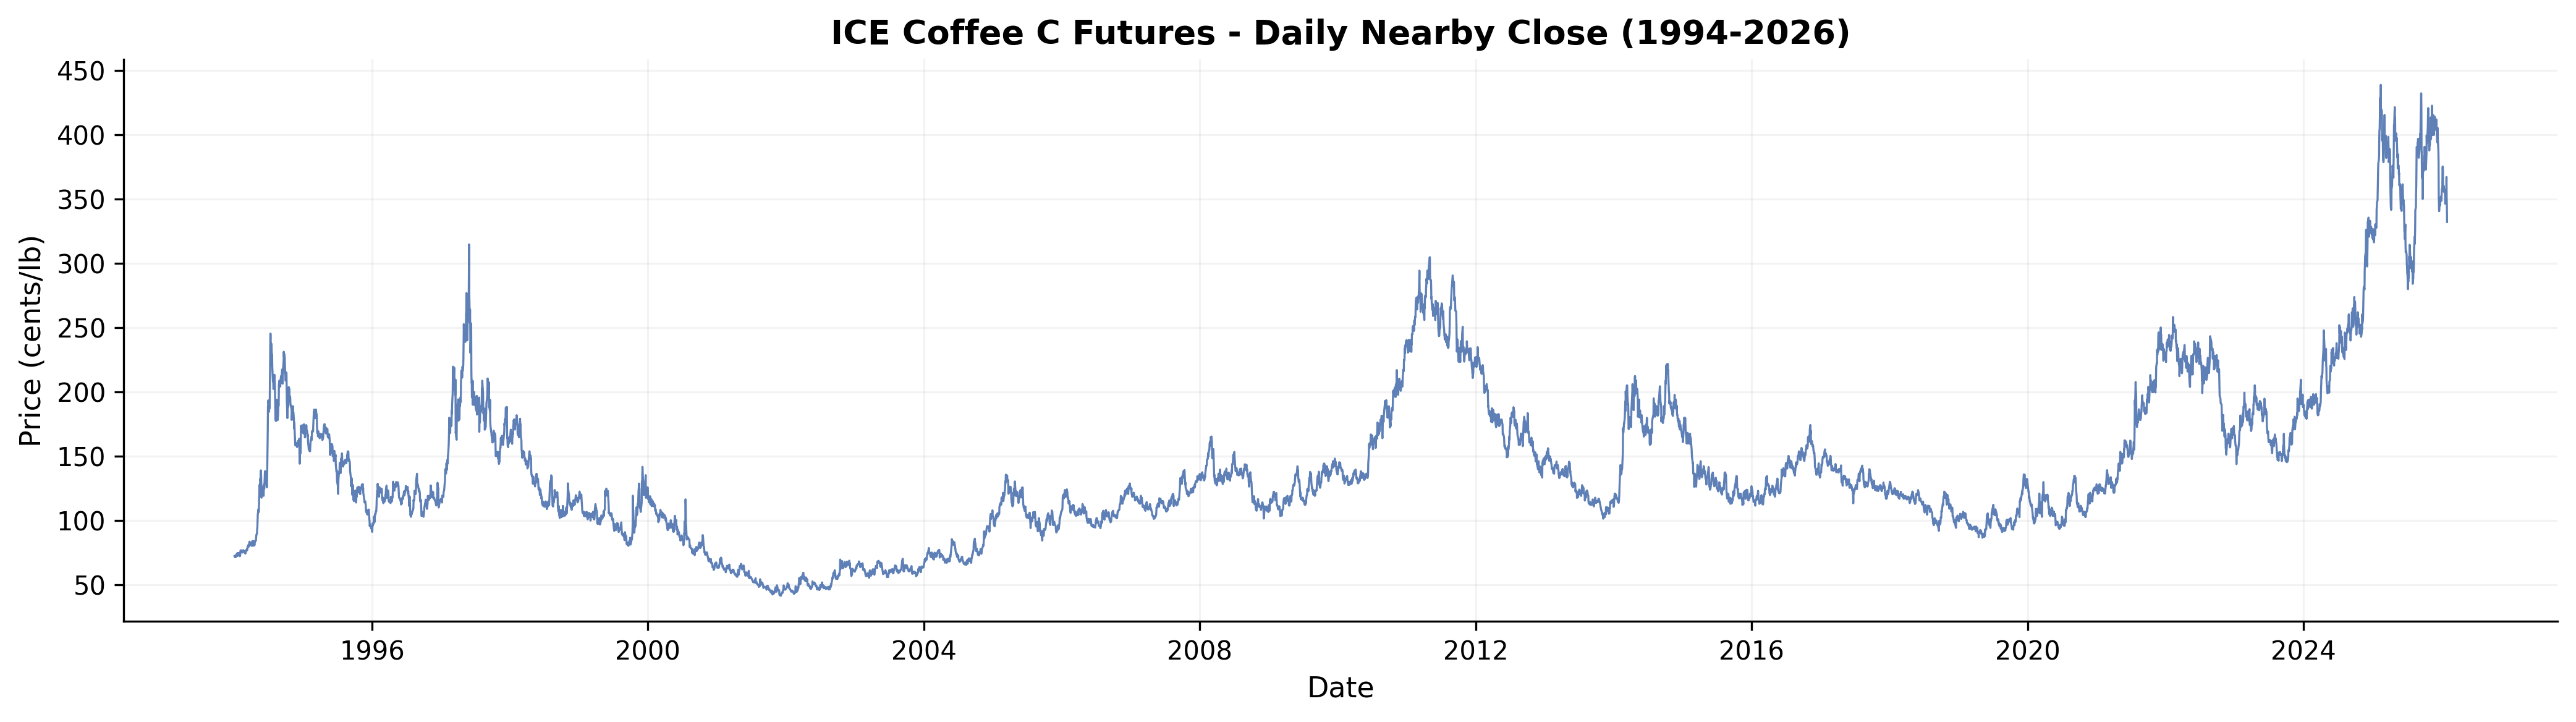
\includegraphics[width=\linewidth]{price_series.png}
  \caption{ICE \emph{Coffee~C} nearby-close daily settlement,
  1994--2026 (8{,}104 trading days). Major regime episodes are
  visible at the 1997 Brazilian frost, the 2010--2011 rally, the
  2014 drought spike, and the 2024--2025 rally past 400 cents/lb.}
  \label{fig:prices}
\end{figure}

% ===================================================================
\section{Forecasting Suite and Backtest Design}
\label{sec:suite}
% ===================================================================

\subsection{Model suite}

Table~\ref{tab:suite} lists the ten models. The suite is constructed
to span the historical landscape of point-forecasting methods, from
the simplest baselines through classical statistical models, a
volatility-aware extension, a structural-decomposition method,
recursive machine-learning approaches, and a contemporary AI
foundation model. Within each category we selected a well-established
representative rather than tuning across alternatives, so the
benchmark tests whether any \emph{family} offers a systematic
advantage over the others rather than whether a particular instance
can be hyperparameter-optimized to win. All models share a
uniform interface: each is wrapped in a class exposing
\verb|predict(context, horizon)| returning a point forecast at every
step of the horizon. Stochastic components (RandomForest at
construction time and any incidental randomness in feature
construction) are seeded; the rest of the suite is deterministic
given fixed inputs (statsforecast and arch use maximum-likelihood
estimation, Granite~TTM is zero-shot, Prophet uses maximum a
posteriori estimation). All implementations rely on standard Python
scientific libraries: \texttt{statsforecast}
\cite{garza2022statsforecast}, \texttt{arch} \cite{sheppard2024arch},
\texttt{Prophet} \cite{taylor2018forecasting}, \texttt{scikit-learn}
\cite{pedregosa2011scikit}, \texttt{statsmodels}
\cite{seabold2010statsmodels}, and the IBM \texttt{tsfm} toolkit
\cite{ekambaram2024ttm}.

\begin{table}[t]
\caption{Forecasting suite}
\label{tab:suite}
\centering
\renewcommand{\arraystretch}{1.1}
\begin{tabular}{@{}ll@{}}
\toprule
\textbf{Category} & \textbf{Model} \\
\midrule
Simple baselines & Naive, Random Walk with Drift (RWD), \\
                 & Theta \cite{assimakopoulos2000theta} \\
Classical statistical & ETS \cite{hyndman2008forecasting}, \\
                      & ARIMA (auto-selected) \cite{box2015time,hyndman2008automatic} \\
Volatility           & GARCH(1{,}1) with AR(1) mean \cite{bollerslev1986generalized} \\
Structural           & Prophet \cite{taylor2018forecasting} \\
Recursive ML         & Ridge \cite{hoerl1970ridge}, Random Forest \cite{breiman2001random} \\
Foundation (zero-shot) & IBM Granite-TimeSeries-TTM-R2 \cite{ekambaram2024ttm} \\
\bottomrule
\end{tabular}
\end{table}

The \emph{GARCH} entry in Table~\ref{tab:suite} is a GARCH(1{,}1)
model with an AR(1) mean and Normal innovations fitted on price
levels, used here as a point-forecast wrapper alongside the rest of
the suite. The GJR-GARCH(1{,}1)-t model that Section~\ref{sec:garch}
specifies for the deployment is a separately-specified variant fitted
to log-returns with Student-$t$ innovations. The two models share a
family name but address different questions: the former contributes a
point forecast to the benchmark, the latter produces calibrated
prediction intervals for deployment.

\subsection{Backtest protocol}

We use a rolling-window backtest with three design parameters:

\begin{itemize}
  \item \textbf{Context window}: 1{,}536 trading days
    ($\approx 6$ years). The Granite-TimeSeries-TTM-R2 release ships
    several zero-shot context-length variants (512, 1024, 1536); we
    use the largest---specifically the \texttt{1536-96-r2} variant,
    with a native 96-step prediction length trimmed to the 63-day
    forecast horizon---so that every model in the suite is given as
    much history as possible while keeping the comparison fair.
  \item \textbf{Horizon}: 63 trading days
    ($\approx 3$ months), long enough to be operationally relevant
    for green-coffee procurement and short enough that point
    forecasts remain defensible.
  \item \textbf{Origins}: 60 evenly-spaced forecast origins
    distributed across the 32-year history
    (Fig.~\ref{fig:origins}). The choice of 60 emerged from a small
    sweep (1, 10, 30, 60); Fig.~\ref{fig:mae-stab} shows the resulting
    mean MAE for each model at each sweep size. The cluster-vs-outlier
    structure of the leaderboard is stable from 30 to 60 origins, and
    within-cluster rankings shuffle by one to three positions while
    all cluster-mean MAE values remain within roughly $0.3$ cents/lb
    of each other in both cases.
\end{itemize}

\begin{figure}[t]
  \centering
  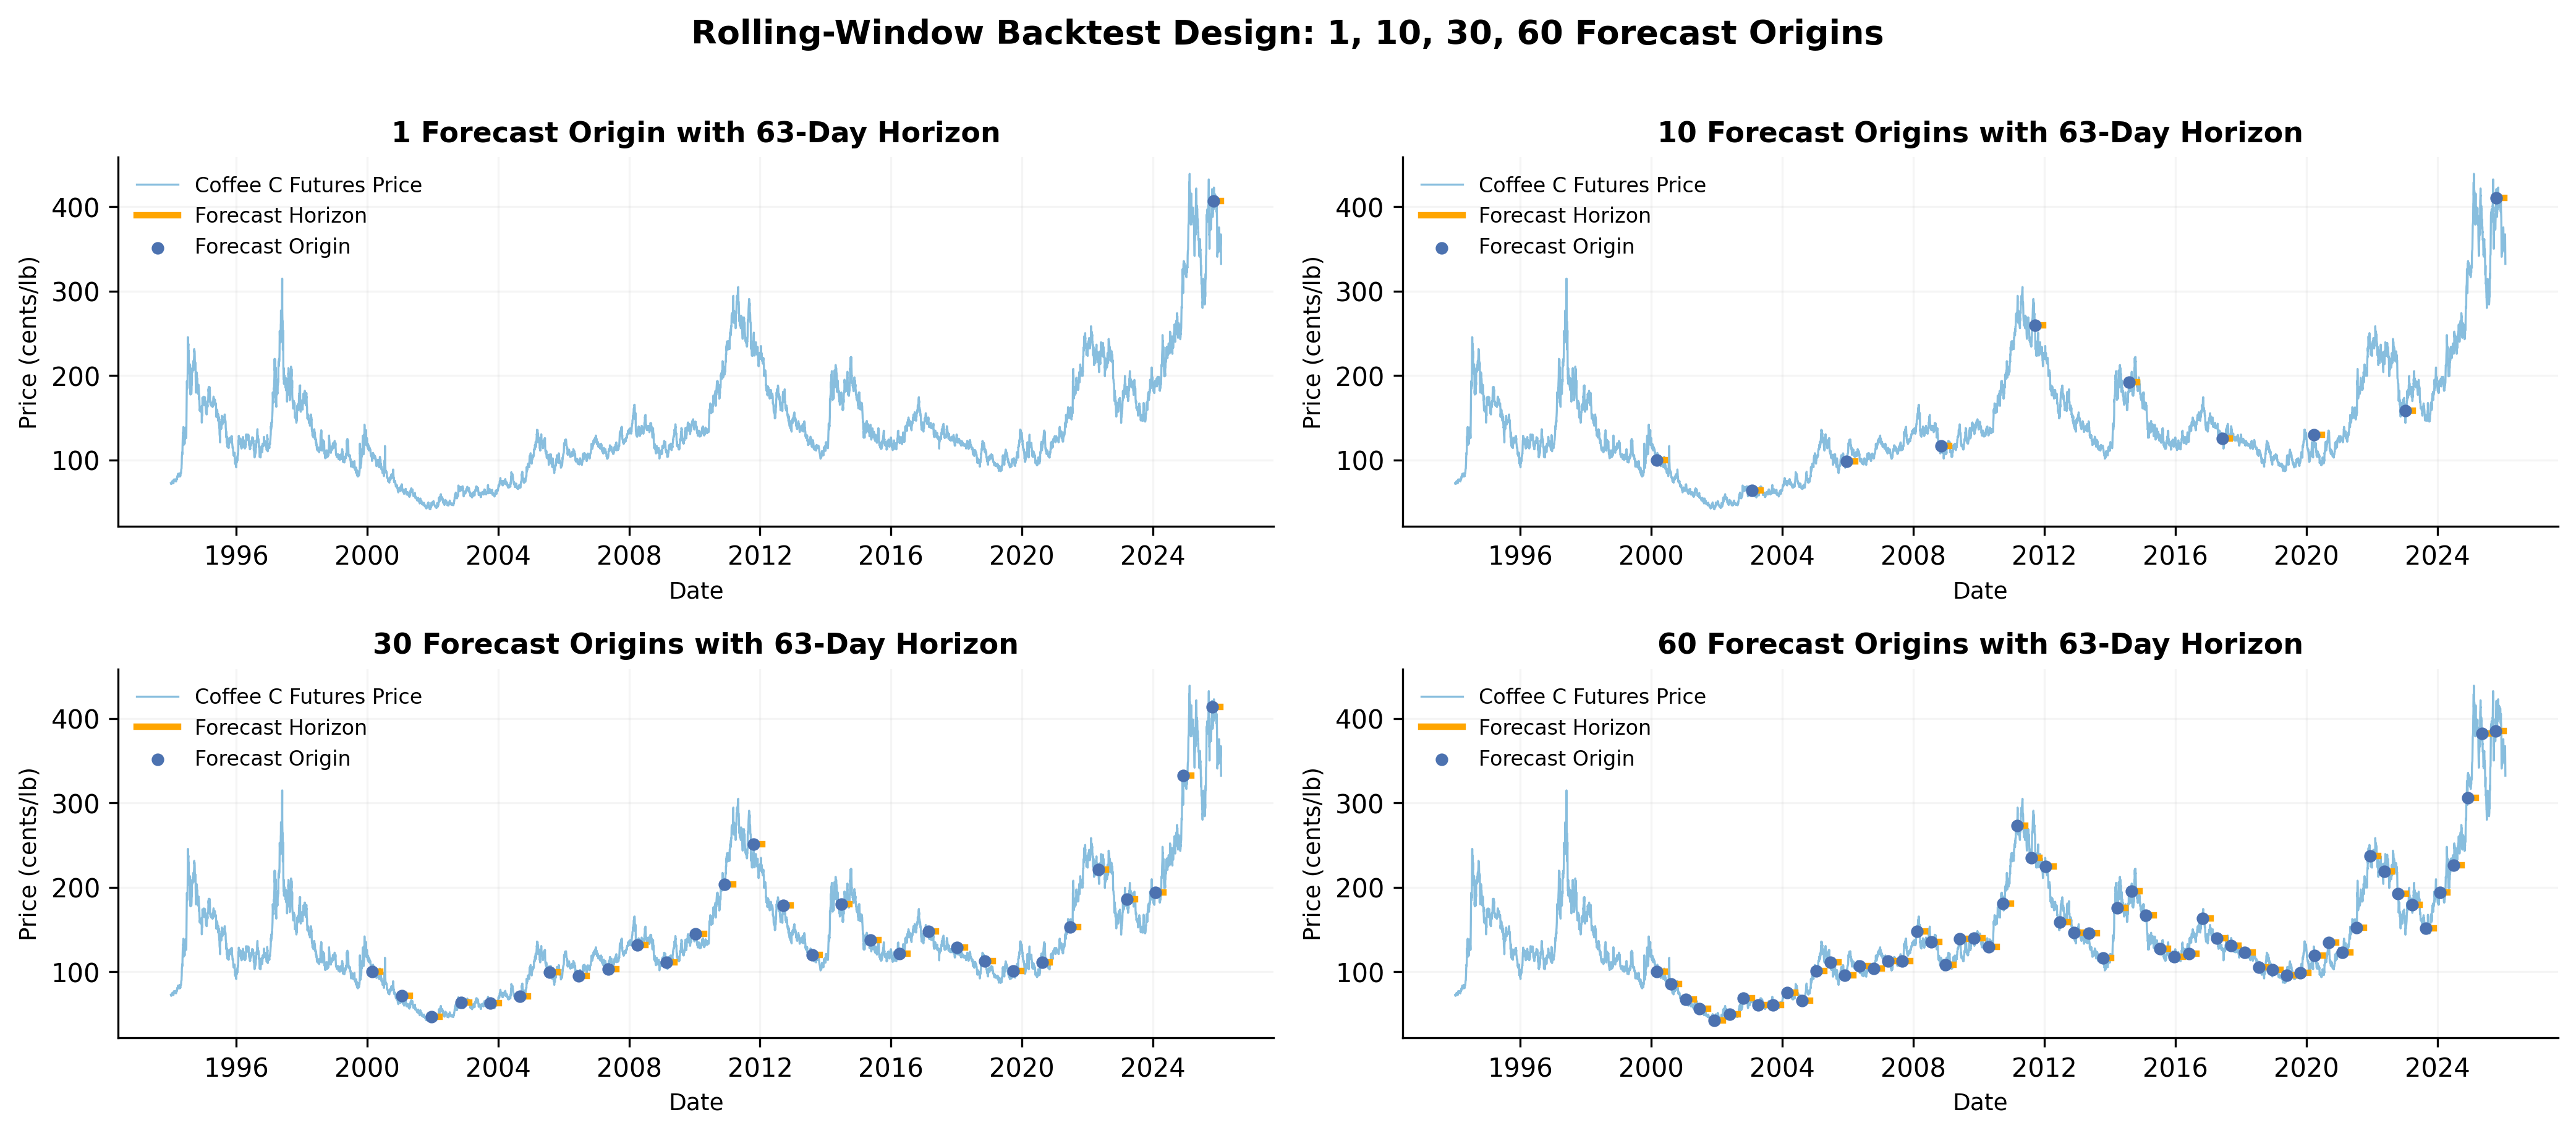
\includegraphics[width=\linewidth]{forecast_origin_coverage.png}
  \caption{Backtest design at the four sweep sizes. Blue circles mark
  forecast origins; orange segments mark the 63-day held-out horizon
  following each. The 60-origin layout (bottom right) is the final
  protocol; the lower sweep sizes are shown for comparison.}
  \label{fig:origins}
\end{figure}

\begin{figure}[t]
  \centering
  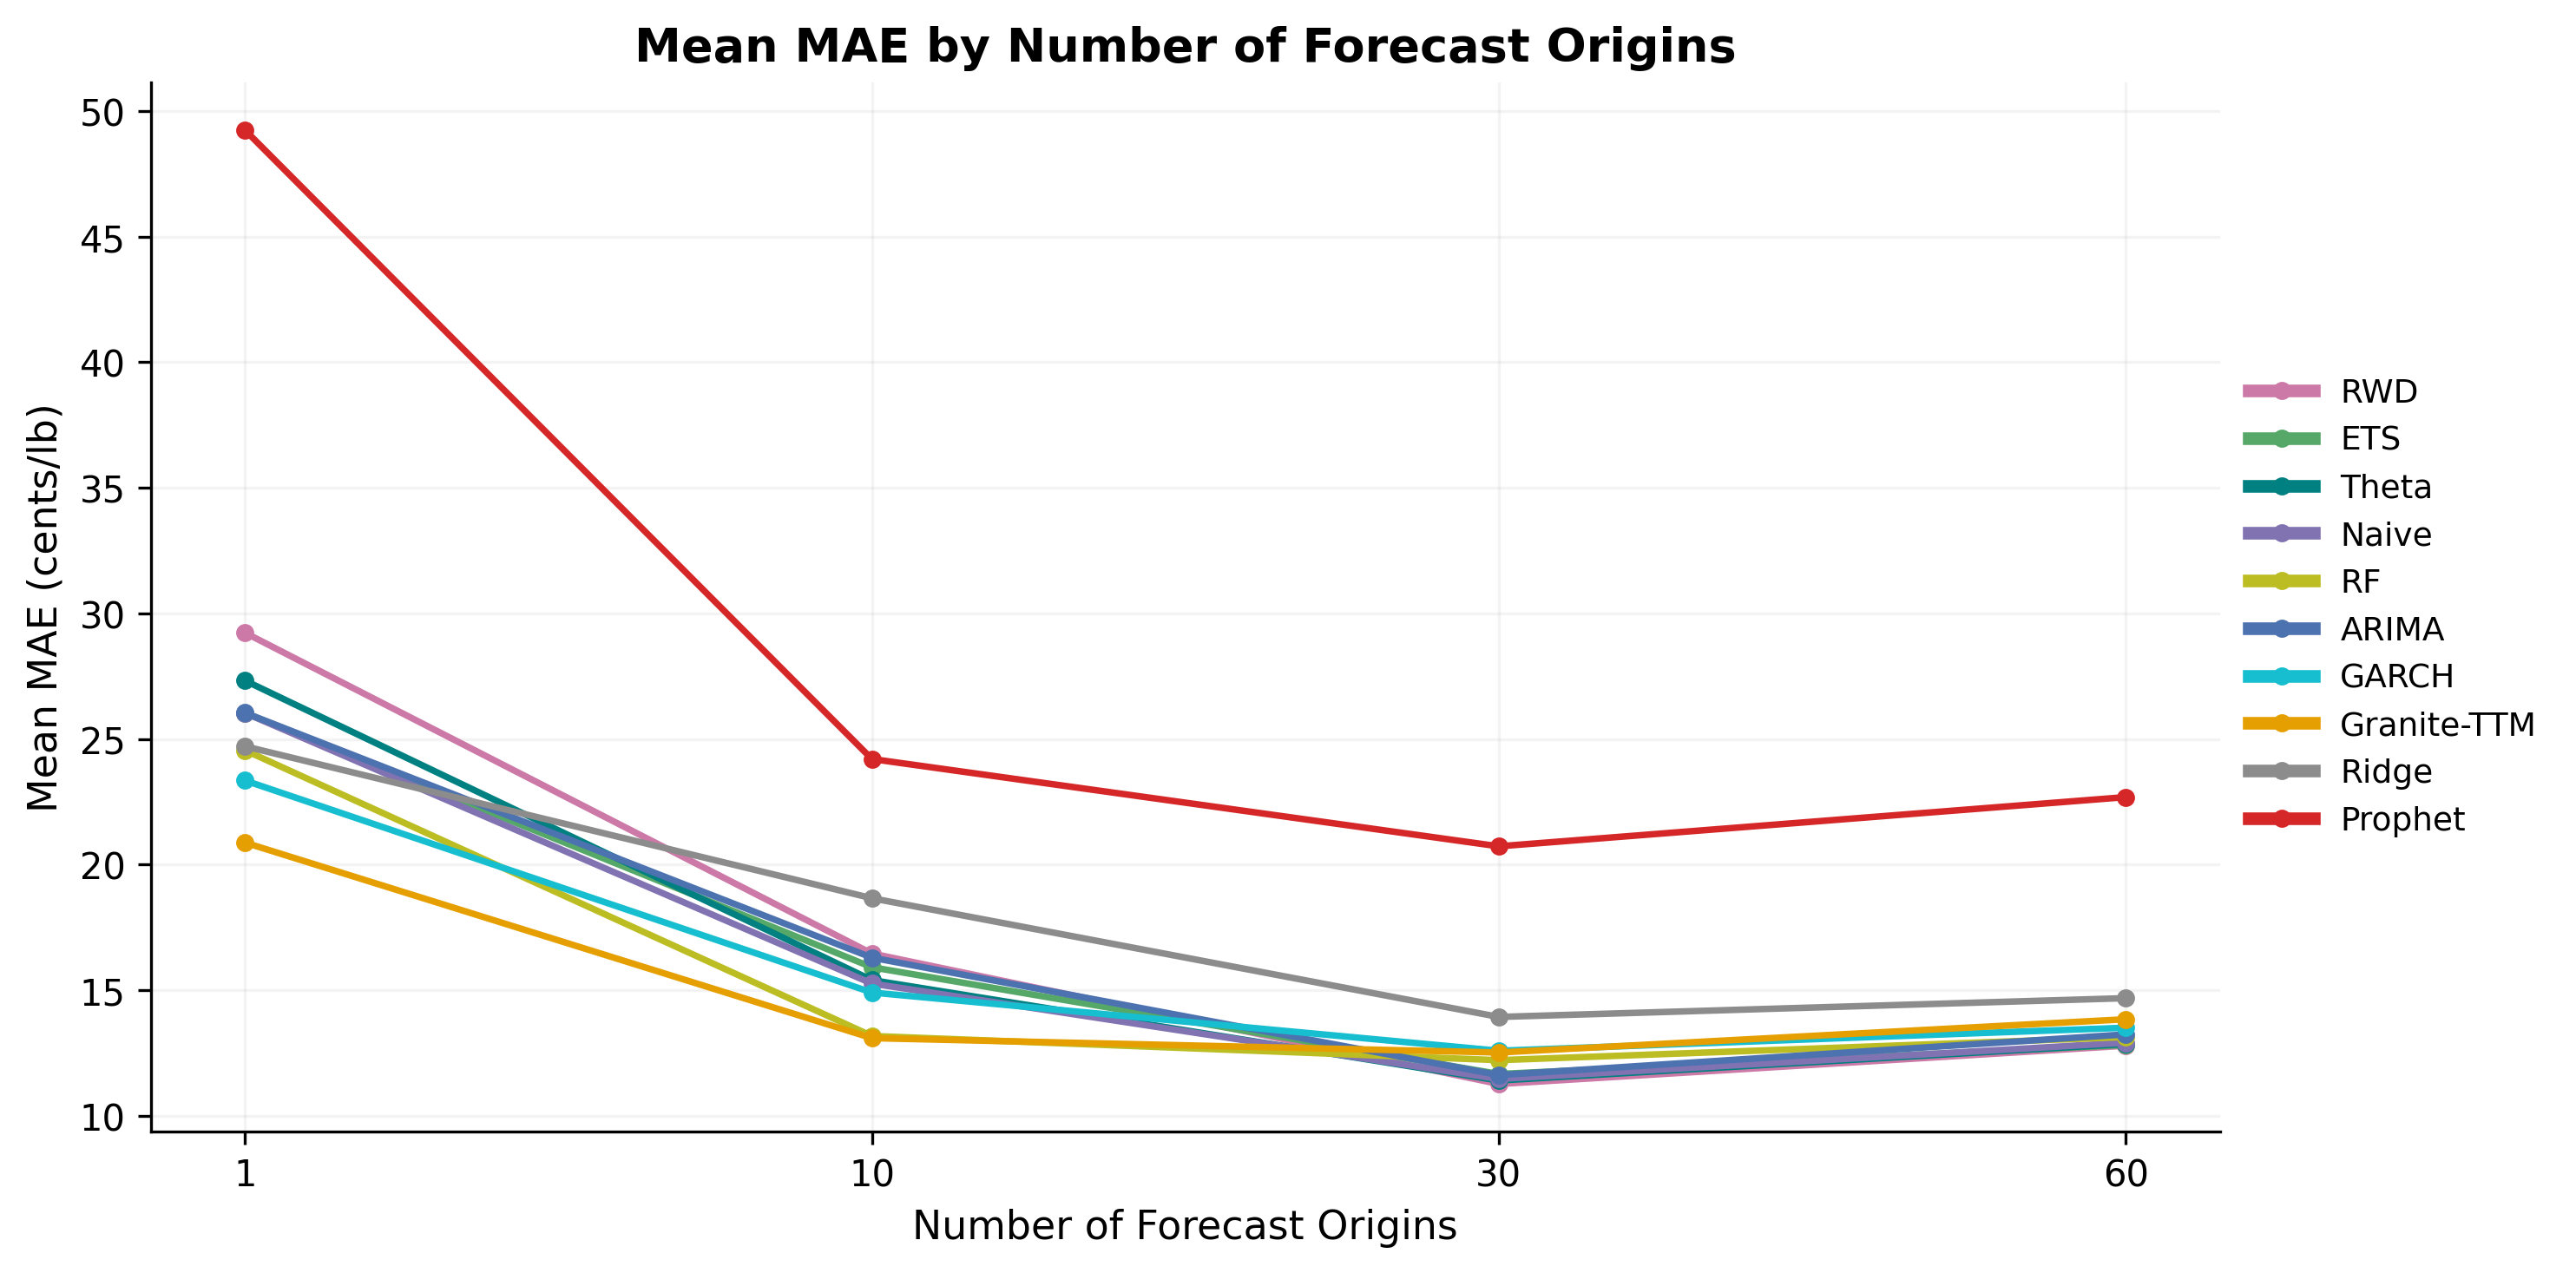
\includegraphics[width=\linewidth]{mae_stabilization.png}
  \caption{Mean MAE by sweep size for all ten models. The nine
  non-Prophet models cluster tightly from 10 origins onward and are
  within roughly $1$ cent/lb of their 60-origin value by 30 origins.
  Prophet remains an outlier at every sweep size.}
  \label{fig:mae-stab}
\end{figure}

At each origin $a$, every model receives the same 1{,}536-day
context $\{y_{a-1535},\dots,y_a\}$ and produces a 63-step forecast.
We compute five forecast-error metrics per (origin, model):
MAE, RMSE, MAPE, sMAPE, and MASE, the last following the
scale-independent definition of Hyndman and Koehler
\cite{hyndman2006another}. The 60-origin protocol yields 600 rows at
the summary level (origins $\times$ models) and 37{,}800 rows at the
per-step level (origins $\times$ models $\times$ horizon steps); the
per-step table is the input to the Diebold-Mariano test and the
Model Confidence Set in Section~\ref{sec:stat-tests}. No model sees
test data during fitting; every origin gets a fresh fit on the
preceding 1{,}536 days.

% ===================================================================
\section{Backtest Results}
\label{sec:backtest}
% ===================================================================

\subsection{Qualitative preview: a single recent window}

Before turning to the 60-origin evaluation, Fig.~\ref{fig:holdout}
shows the 10-model overlay on the most recent 63-day window with the
realized price path in black. Every model produces a visually
plausible trajectory, and several track the realized path closely on
this particular window---including Granite~TTM, which has the lowest
MAE here. The 60-origin evaluation that follows returns a very
different ranking, which is itself a useful warning about reading too
much into any single window.

\begin{figure}[t]
  \centering
  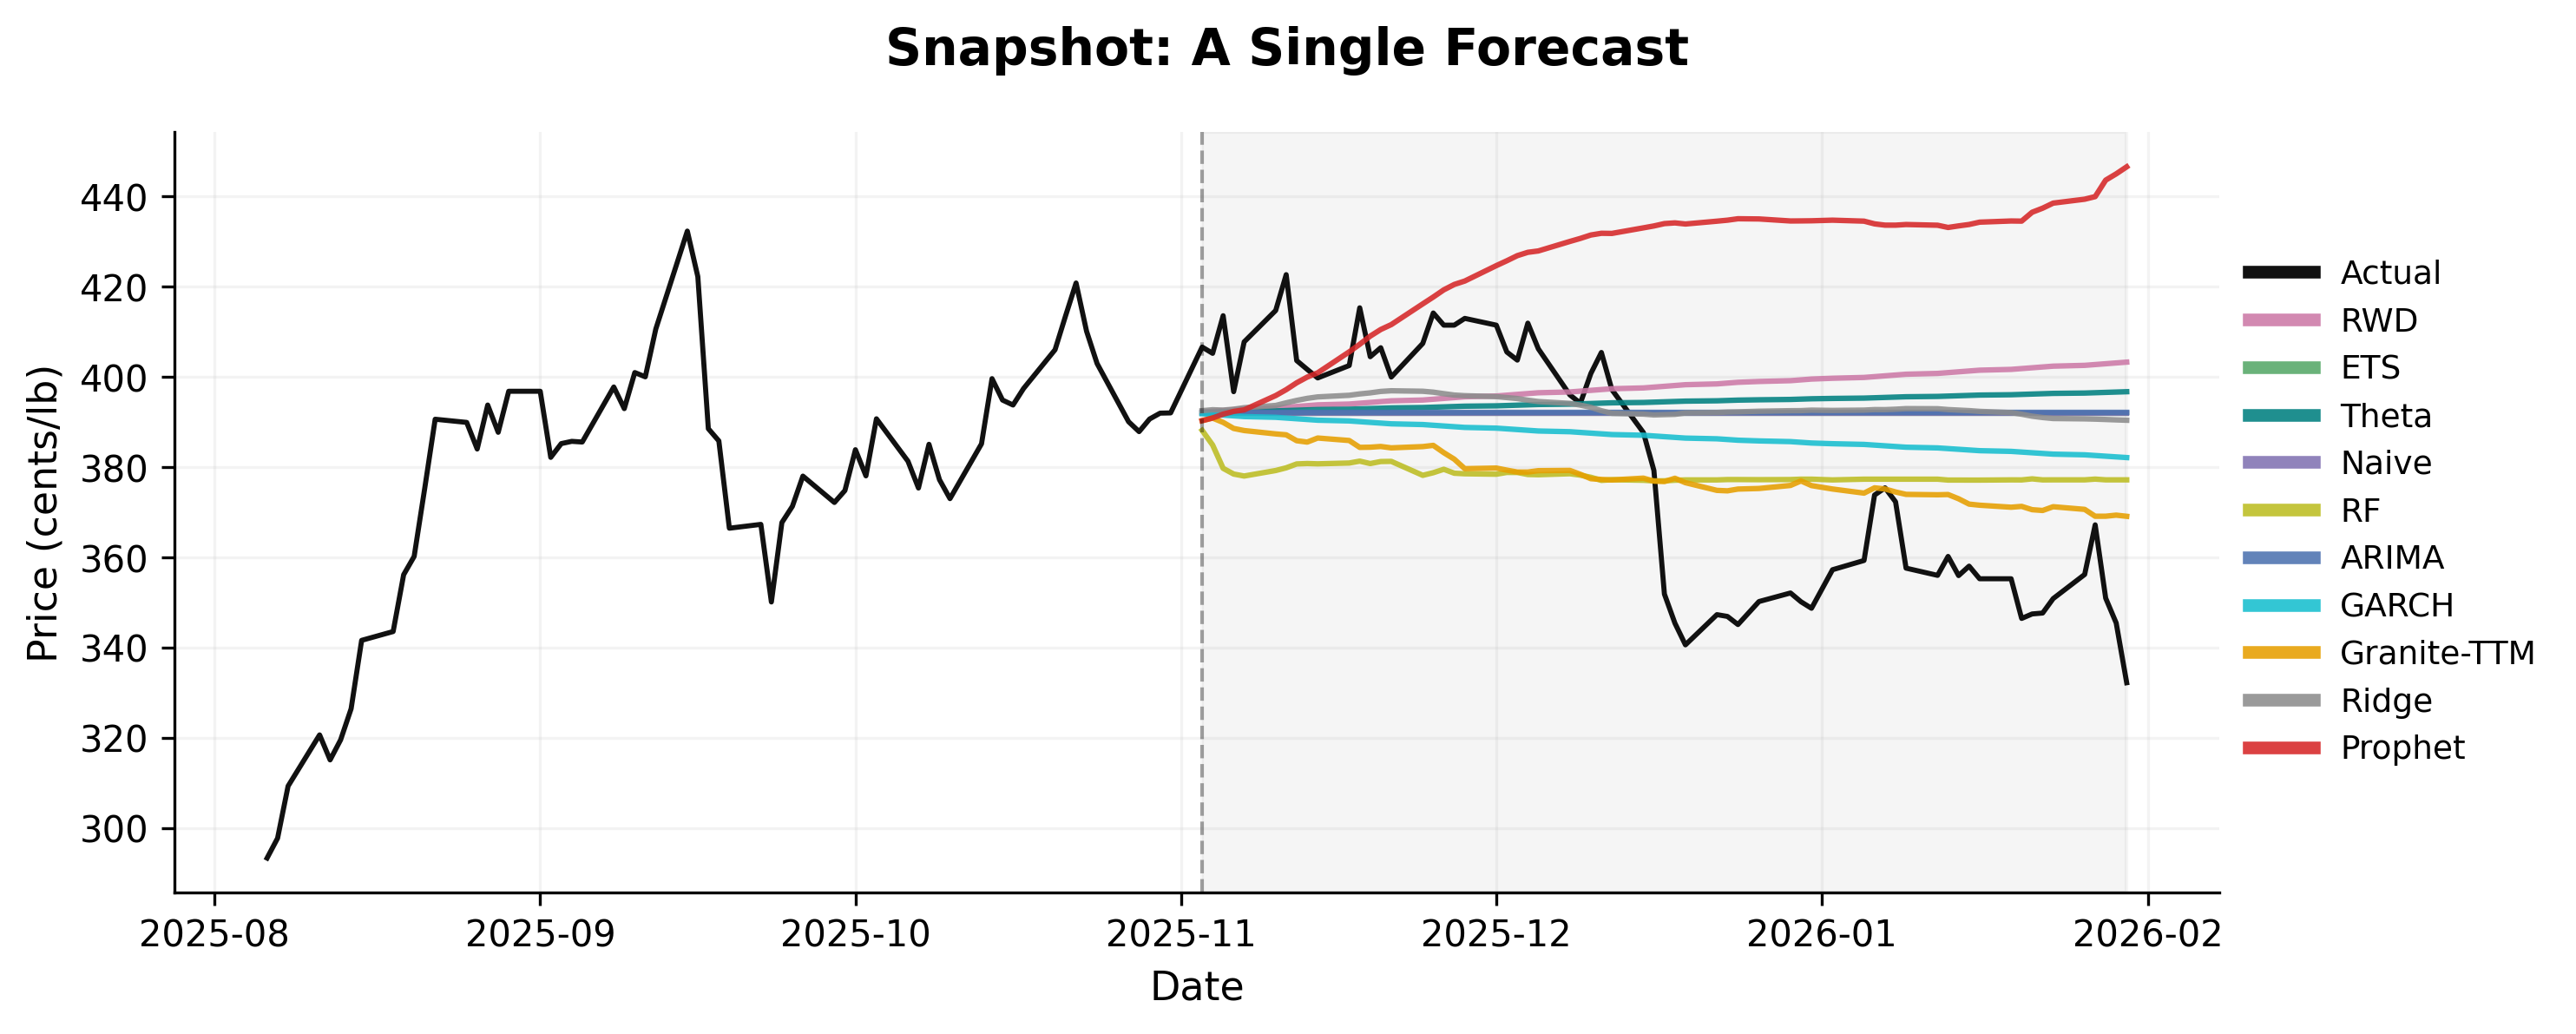
\includegraphics[width=\linewidth]{coffee_holdout_plot.png}
  \caption{Qualitative preview: 10-model forecasts on the most recent
  63-day window, overlaid against the realized price path (black).
  The shaded region marks the held-out forecast horizon. Every model
  is visually plausible on this single window; the 60-origin
  evaluation that follows tells the rigorous story.}
  \label{fig:holdout}
\end{figure}

\subsection{Leaderboard at 60 origins}

Table~\ref{tab:leaderboard} reports mean per-origin error metrics at
the 60-origin scale, sorted by MAE. The arithmetic leader is the
random walk with drift, followed by the other simple baselines (ETS,
Theta, Naive) within $0.15$~MAE of it. The two machine-learning
models (Random Forest, Ridge) and the AI foundation model
(Granite~TTM) all rank below the simple baselines on mean MAE;
increased model complexity does not translate into lower
point-forecast error on this series. Prophet sits well outside the
cluster.

\begin{table}[t]
\caption{60-origin mean error metrics, sorted by MAE}
\label{tab:leaderboard}
\centering
\renewcommand{\arraystretch}{1.1}
\begin{tabular}{@{}lcccc@{}}
\toprule
\textbf{Model} & \textbf{MAE} & \textbf{RMSE} & \textbf{MASE} & \textbf{sMAPE} \\
\midrule
RWD          & 12.79 & 14.84 &  6.10 & 0.083 \\
ETS          & 12.82 & 14.89 &  6.11 & 0.085 \\
Theta        & 12.86 & 14.93 &  6.13 & 0.085 \\
Naive        & 12.91 & 14.99 &  6.15 & 0.085 \\
RF           & 13.13 & 15.19 &  6.28 & 0.087 \\
ARIMA        & 13.24 & 15.39 &  6.28 & 0.085 \\
GARCH        & 13.51 & 15.74 &  6.50 & 0.090 \\
Granite-TTM  & 13.84 & 16.09 &  6.55 & 0.092 \\
Ridge        & 14.68 & 17.16 &  6.87 & 0.101 \\
Prophet      & 22.69 & 24.99 & 10.60 & 0.152 \\
\bottomrule
\end{tabular}
\end{table}

\subsection{Distribution of per-origin MAE}

Mean metrics sort the models but can hide right tails; a model with
average behavior most of the time but occasional collapses will look
worse than it deserves, and vice versa. Fig.~\ref{fig:mae-box} shows
the full per-origin MAE distribution at scale 60. Boxes are sorted by
median, the mean is overlaid as a black diamond, and the nine
indistinguishable cluster models are colored neutral with Prophet in
red.

\begin{figure}[t]
  \centering
  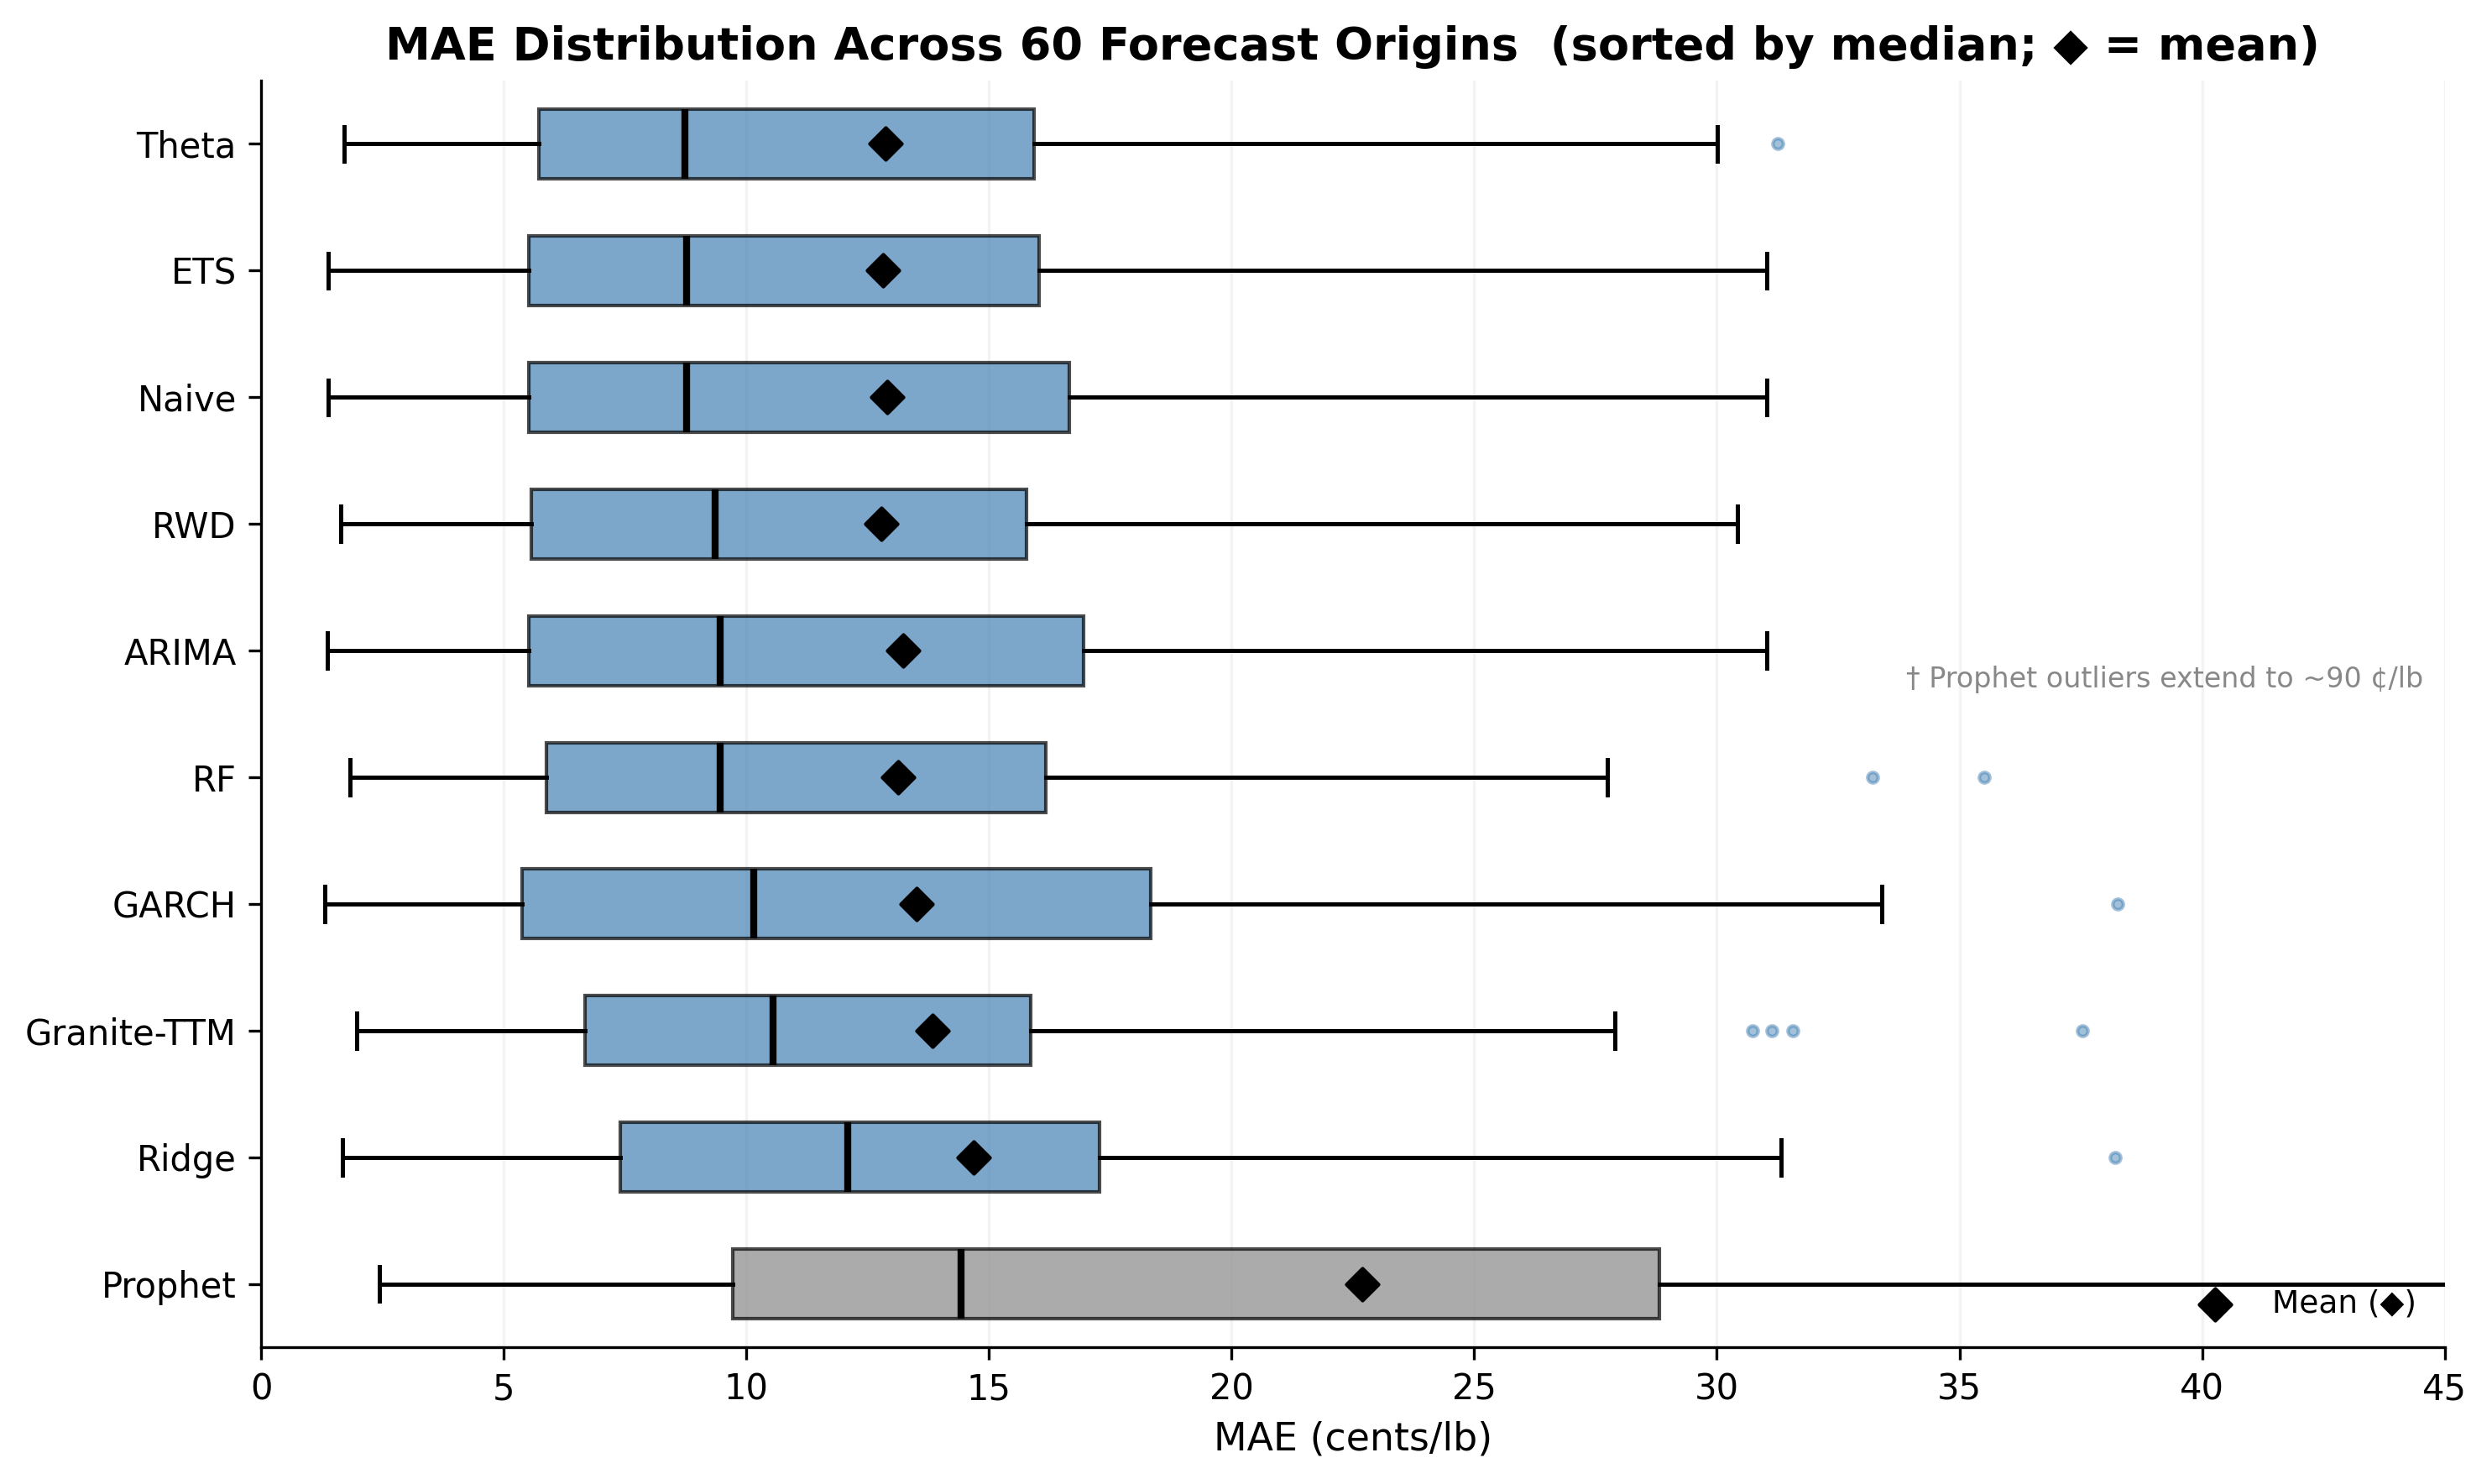
\includegraphics[width=\linewidth]{model_comparison_60.png}
  \caption{MAE distribution across 60 forecast origins, sorted by
  median MAE (worst at top). Diamonds mark the mean. The nine
  MCS-retained models (steelblue) have heavily overlapping
  interquartile ranges; Prophet, the only MCS-eliminated model
  (gray), sits well to the right of the cluster with a much heavier
  right tail.}
  \label{fig:mae-box}
\end{figure}

Two patterns are visible. First, the IQRs of the nine non-Prophet
models overlap heavily---visual evidence for the statistical tie
formalized in Section~\ref{sec:stat-tests}. Second, the
mean-minus-median gap for the nine cluster models is similar in
magnitude (roughly $2.6$--$4.1$~cents/lb), so no cluster model is
distinguished by a particularly asymmetric distribution. Prophet's
mean-minus-median gap is $8.3$~cents/lb, reflecting catastrophic
tail behavior on a subset of origins rather than a uniformly higher
error level.

\subsection{Granite~TTM versus RWD across origins}

The boxplot in Fig.~\ref{fig:mae-box} already shows that Granite~TTM
has a higher \emph{mean} and \emph{median} MAE than RWD, with a
mean-minus-median gap of $3.3$~cents/lb that is in the middle of
the cluster range. A natural follow-up is whether the
underperformance is concentrated in a few collapsed windows or
distributed across the historical record.
Fig.~\ref{fig:ttm-rwd} answers this directly by overlaying the
per-origin MAE of Granite~TTM and RWD at each of the 60 origins. The
orange-shaded area marks origins where Granite exceeds RWD; the area
is nearly continuous, and Granite achieves lower MAE at only 16 of 60
origins. The foundation model underperforms the drift baseline not
because of a small number of collapses but through a steady positive
bias across the historical record.

\begin{figure}[t]
  \centering
  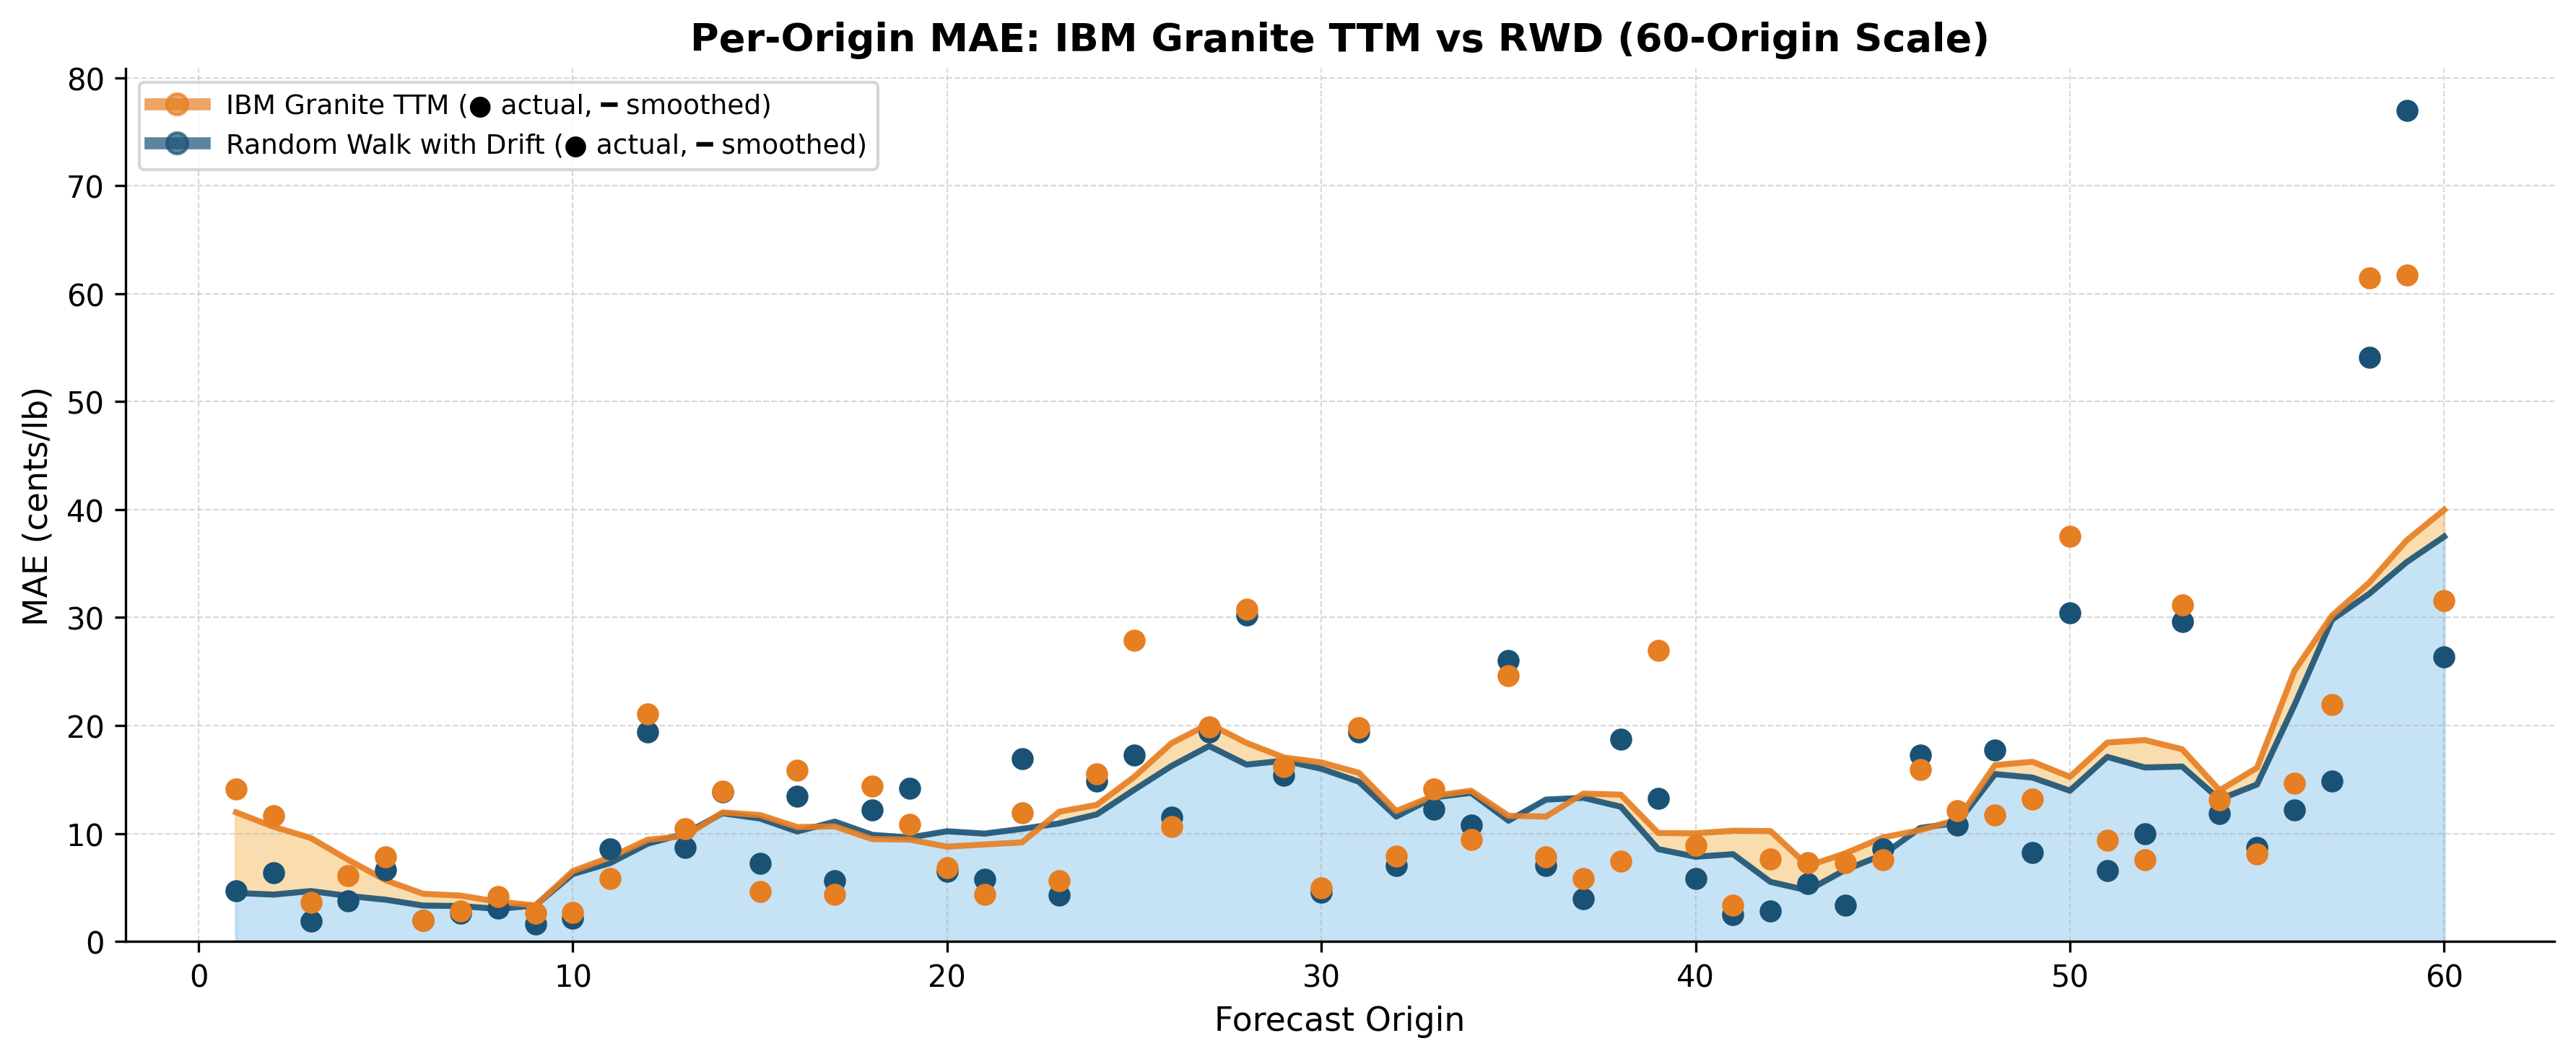
\includegraphics[width=\linewidth]{IBM_vs_RWD.png}
  \caption{Per-origin MAE: IBM Granite~TTM versus RWD across 60
  origins. Markers are observed values; lines are smoothed
  trends. Granite achieves lower MAE at only 16 of 60 origins;
  the orange band is the excess error above RWD.}
  \label{fig:ttm-rwd}
\end{figure}

% ===================================================================
\section{Statistical Tests}
\label{sec:stat-tests}
% ===================================================================

The leaderboard rankings are descriptive and do not distinguish
sampling noise from real differences in predictive accuracy. We use
two complementary tools to do so: the Diebold-Mariano test pairwise
against the RWD baseline, and the Model Confidence Set as a joint
test on the full suite.

\subsection{Diebold-Mariano test versus RWD}

The DM test \cite{diebold1995comparing} addresses the null that two
forecasts have equal predictive accuracy. We use the per-origin MAE
loss as the comparison statistic and estimate the HAC variance
across origins with the Bartlett kernel and the Newey-West
\cite{newey1994automatic} rule-of-thumb bandwidth
$\lfloor 4(T/100)^{2/9}\rfloor$. We apply the Harvey-Leybourne-Newbold
\cite{harvey1997testing} small-sample correction: the statistic is
multiplied by $\sqrt{(T+1-2h+h(h-1)/T)/T}$ (here $h=1$, so by
$\sqrt{(T-1)/T}$) and referenced against the $t_{T-1}$ distribution
rather than $\mathcal{N}(0,1)$.

Three patterns appear. The top-tier simple models (ETS, Theta, Naive)
do not differ significantly from RWD ($p > 0.4$); their gaps fall
within sampling noise. Granite~TTM is significantly worse than RWD
at the 5\% level (DM~$=+2.35$, $p = 0.022$), and Ridge at the same
level (DM~$=+2.04$, $p = 0.046$). Prophet is rejected at the 0.1\%
level (DM~$=+4.53$, $p < 0.001$). GARCH sits just over the 10\%
threshold (DM~$=+1.76$, $p = 0.083$).

\subsection{Model Confidence Set}

DM compares each model to a fixed baseline and does not correct for
multiple comparisons; running nine pairwise tests against RWD inflates
the Type~I error rate. The Model Confidence Set \cite{hansen2011model}
addresses this by returning a \emph{set} of models statistically
indistinguishable from the best at significance $\alpha$. The
procedure starts with all ten models, computes the max-$t$ statistic
across centered loss differentials, bootstraps the null distribution
(circular block bootstrap, $B = 5000$, block size 5), eliminates the
model with the largest $t$-statistic if $p \le \alpha$, and repeats
until no further elimination is possible. p-values reported for
eliminated models are monotonically adjusted across elimination
steps, so an MCS p-value for a later-eliminated model cannot fall
below that of an earlier-eliminated one.

At $\alpha = 0.10$, the MCS retains nine of the ten models: Naive,
RWD, Theta, ETS, ARIMA, GARCH, Ridge, RF, and Granite-TTM. Only
Prophet is eliminated, with MCS $p = 0.009$. The retained set spans
every category in the suite, including the foundation model.

\subsection{Reconciling DM and MCS}

The two tests can look superficially contradictory: DM rejects equal
accuracy between RWD and Granite (and Ridge) at the 5\% level, while
MCS keeps both in the confidence set with $p = 1.000$. The gap
reflects multiple-comparisons correction. A Bonferroni adjustment to
the nine pairwise DM tests---$\alpha/9 \approx 0.006$ for an overall
5\% rate---would eliminate the marginal Granite-TTM and Ridge
significances and leave only Prophet rejected, which is the
conclusion the MCS reaches by construction. With ten models the joint
test is the appropriate primary tool; DM is a familiar pairwise
summary that supplements rather than contradicts it.

A caveat on power: $T = 60$ origins is on the small side for MCS (the
Hansen-Lunde-Nason simulations use $T = 100$--$500$), so a
wider-than-true MCS is partly a power story. The qualitative
finding---Prophet eliminated, the remaining nine retained---is
robust, but the surviving set could plausibly shrink with more
origins.

\begin{figure}[t]
  \centering
  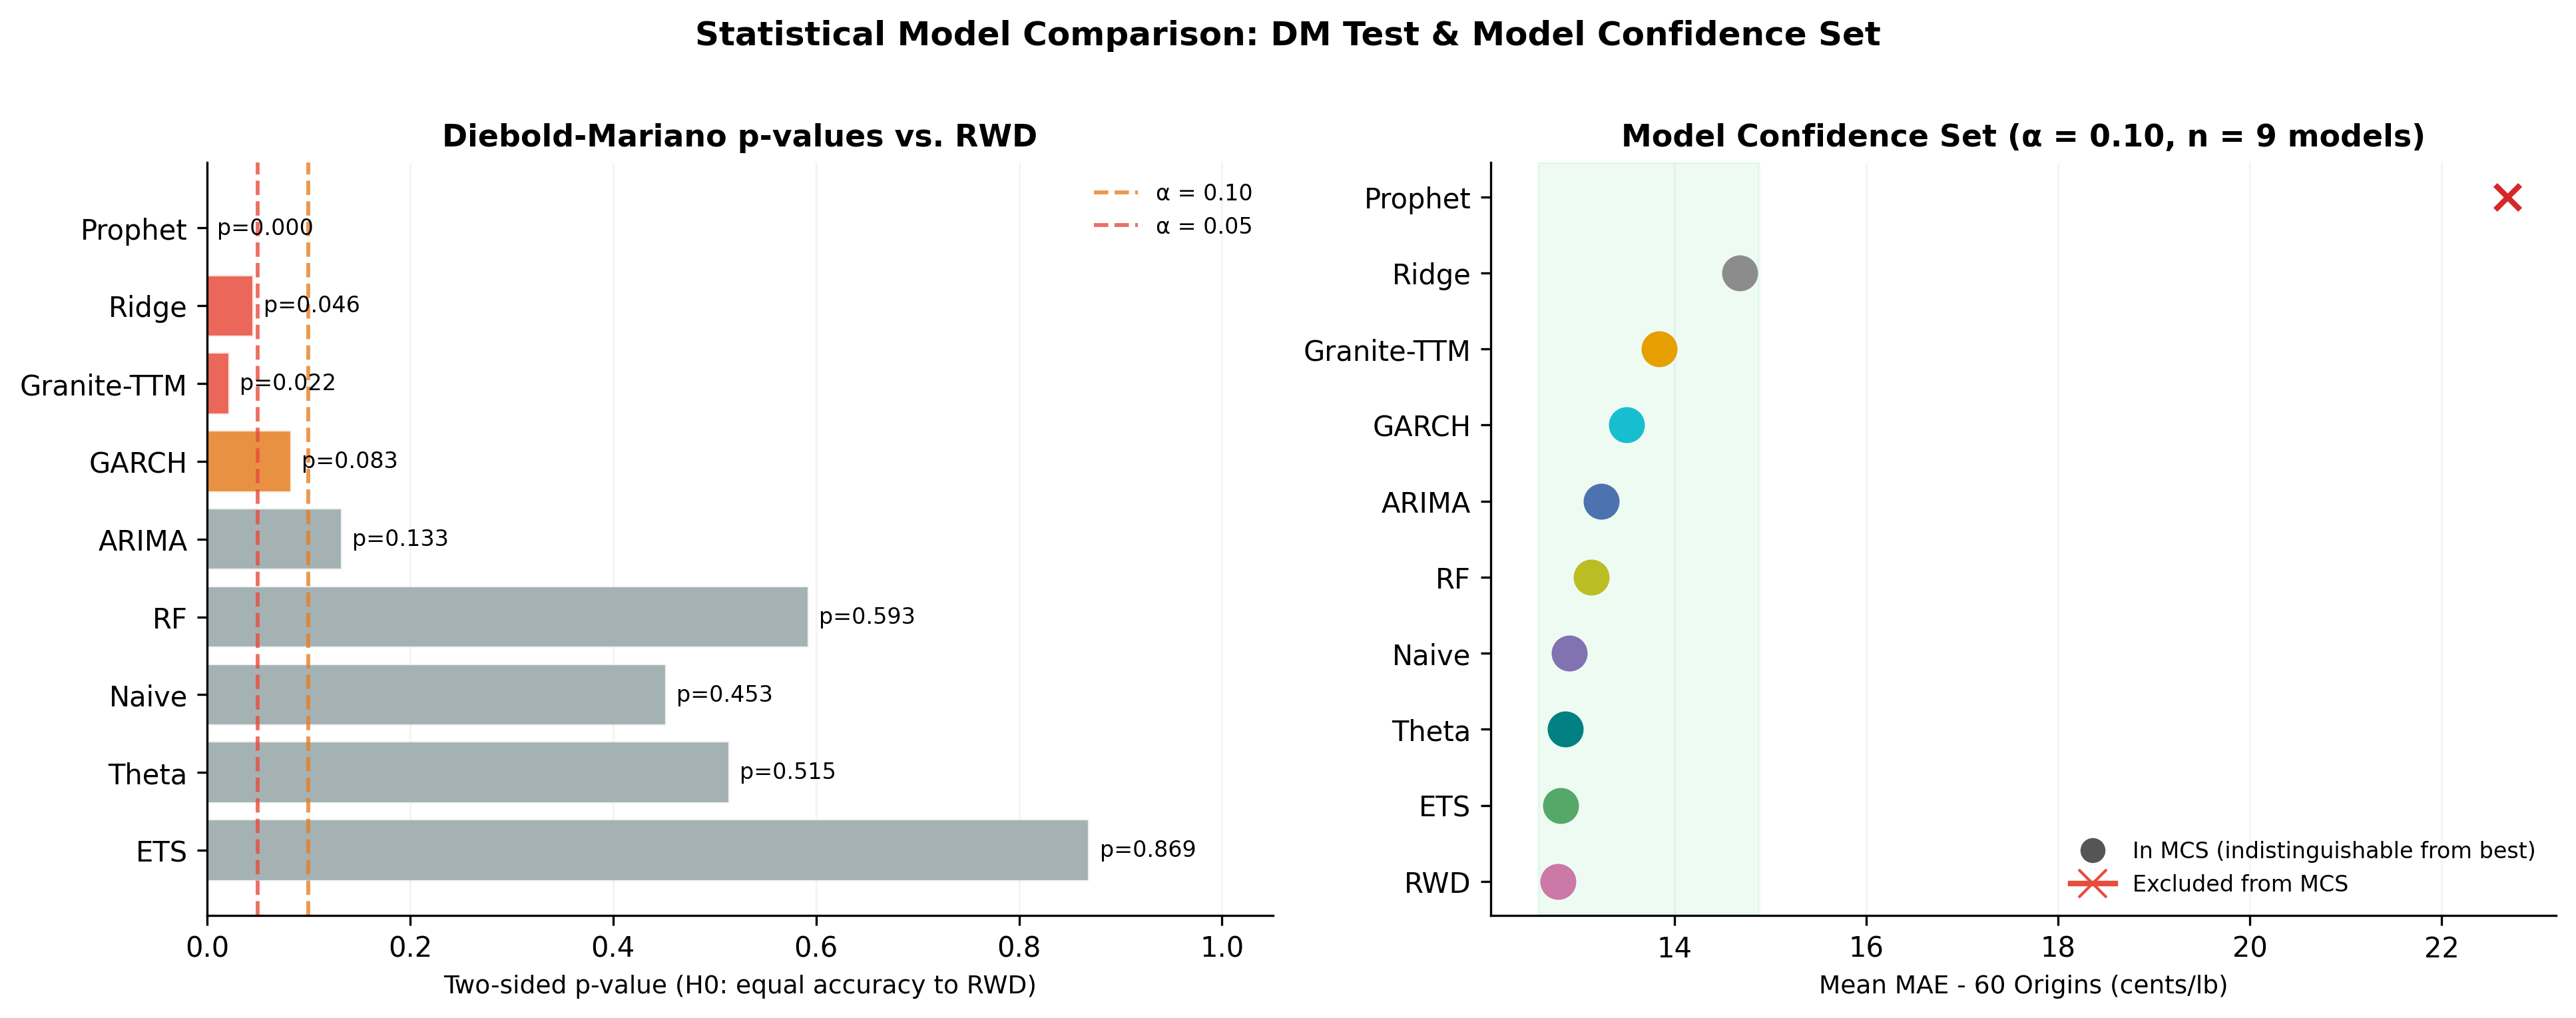
\includegraphics[width=\linewidth]{dm_mcs.png}
  \caption{Statistical model comparison.
  \emph{Left}: Diebold-Mariano p-values versus RWD; bars colored by
  significance threshold ($p < 0.05$ in red, $p < 0.10$ in orange).
  \emph{Right}: Model Confidence Set at $\alpha = 0.10$; survivors
  marked as filled circles, Prophet (the sole eliminated model) as a
  red cross. The green band shows the range of mean MAE across MCS
  survivors.}
  \label{fig:dm-mcs}
\end{figure}

\subsection{Reading}

Nine of ten models---spanning random-walk baselines, classical
statistical models, a volatility model, recursive ML, and a
foundation model---are jointly indistinguishable from the best at
$\alpha = 0.10$. The leaderboard in Table~\ref{tab:leaderboard} is
therefore descriptive rather than a true ranking: RWD is not "the
winner" but the arithmetic leader of a cluster of
statistically-equivalent models, and the benchmark does not have
enough resolving power to single one out. A diverse 10-model suite
that includes a pretrained foundation model with a six-year context
window cannot statistically distinguish itself from a naive drift
forecaster on this series.

% ===================================================================
\section{Forecastability Diagnostics}
\label{sec:forecastability}
% ===================================================================

The benchmark tie has two possible readings. Either our suite is the
wrong instrument and a different class of models would extract
structure ours misses, or the series itself carries little
exploitable structure at this horizon. We test the second reading
directly with a battery of diagnostics applied to the series alone,
independent of any forecasting model. Table~\ref{tab:diagnostics}
collects all results; the prose below groups them thematically. We
give primary weight to the standard finance-econometrics battery
(stationarity, linear predictability, long memory) and supplement it
with three exploratory metrics from the nonlinear-dynamics and
signal-processing literatures as an independent cross-check.

\begin{table}[t]
\caption{Forecastability diagnostics on coffee log-returns}
\label{tab:diagnostics}
\centering
\renewcommand{\arraystretch}{1.15}
\begin{tabular}{@{}p{0.30\linewidth}p{0.32\linewidth}p{0.28\linewidth}@{}}
\toprule
\textbf{Test} & \textbf{Null} & \textbf{Result} \\
\midrule
\multicolumn{3}{l}{\emph{Stationarity (on prices / on log-returns)}} \\
ADF \cite{dickey1979distribution}            & Unit root           & $p = 0.557$ / $p < 10^{-90}$ \\
KPSS \cite{kwiatkowski1992testing}           & Stationary          & $p < 0.01$ / $p > 0.10$ \\
Phillips-Perron \cite{phillips1988testing}   & Unit root           & $p = 0.418$ / $p < 10^{-90}$ \\
\midrule
\multicolumn{3}{l}{\emph{Linear predictability of log-returns}} \\
Ljung-Box ($L{=}10,20$) \cite{ljung1978measure}        & No autocorrelation  & $p \approx 0.006$; $\overline{|\hat\rho|} \approx 0.013$ \\
Lo-MacKinlay VR ($q{=}2,\dots,32$) \cite{lo1988stock}  & Random walk         & Fail to reject at all $q$ \\
\midrule
\multicolumn{3}{l}{\emph{Long memory}} \\
Hurst exponent \cite{hurst1951long}          & ---                 & $H = 0.535$ \\
Lo's modified $V_n$ \cite{lo1991long}        & No long memory      & $V_n = 1.137 \in [0.809, 1.862]$ \\
\midrule
\multicolumn{3}{l}{\emph{Exploratory metrics on log-returns}} \\
Spectral predictability $\Omega$ \cite{wang2025spectral}      & ---  & $\Omega \approx 0.05$ (near floor) \\
Permutation entropy \cite{bandt2002permutation}               & ---  & $\approx 1.00$ (near ceiling) \\
Rosenstein $\lambda$ vs.\ surrogate \cite{rosenstein1993practical,theiler1992testing}  & Shuffled-return null & $p = 0.97$ \\
\bottomrule
\end{tabular}
\end{table}

\subsection{Stationarity}
\label{sec:stationarity}

Several diagnostics (variance ratio, Hurst with R/S, the Lyapunov
reconstruction) require a stationary input, and the GARCH deployment
in Section~\ref{sec:garch} works in log-returns for the same reason.
Fig.~\ref{fig:prices-vs-returns} shows the price level and its
log-returns side by side. Three complementary unit-root tests agree:
on prices, ADF and Phillips-Perron fail to reject the unit-root null
while KPSS rejects stationarity; on log-returns the directions flip,
with ADF and PP rejecting at $p < 10^{-90}$ and KPSS failing to
reject. The confirmatory design---ADF and Phillips-Perron paired with
the oppositely-directed KPSS---eliminates the standard "low-power
ADF" critique, and the Phillips-Perron non-parametric correction is
robust to the heteroskedasticity that Section~\ref{sec:garch}
formally documents.

\begin{figure}[t]
  \centering
  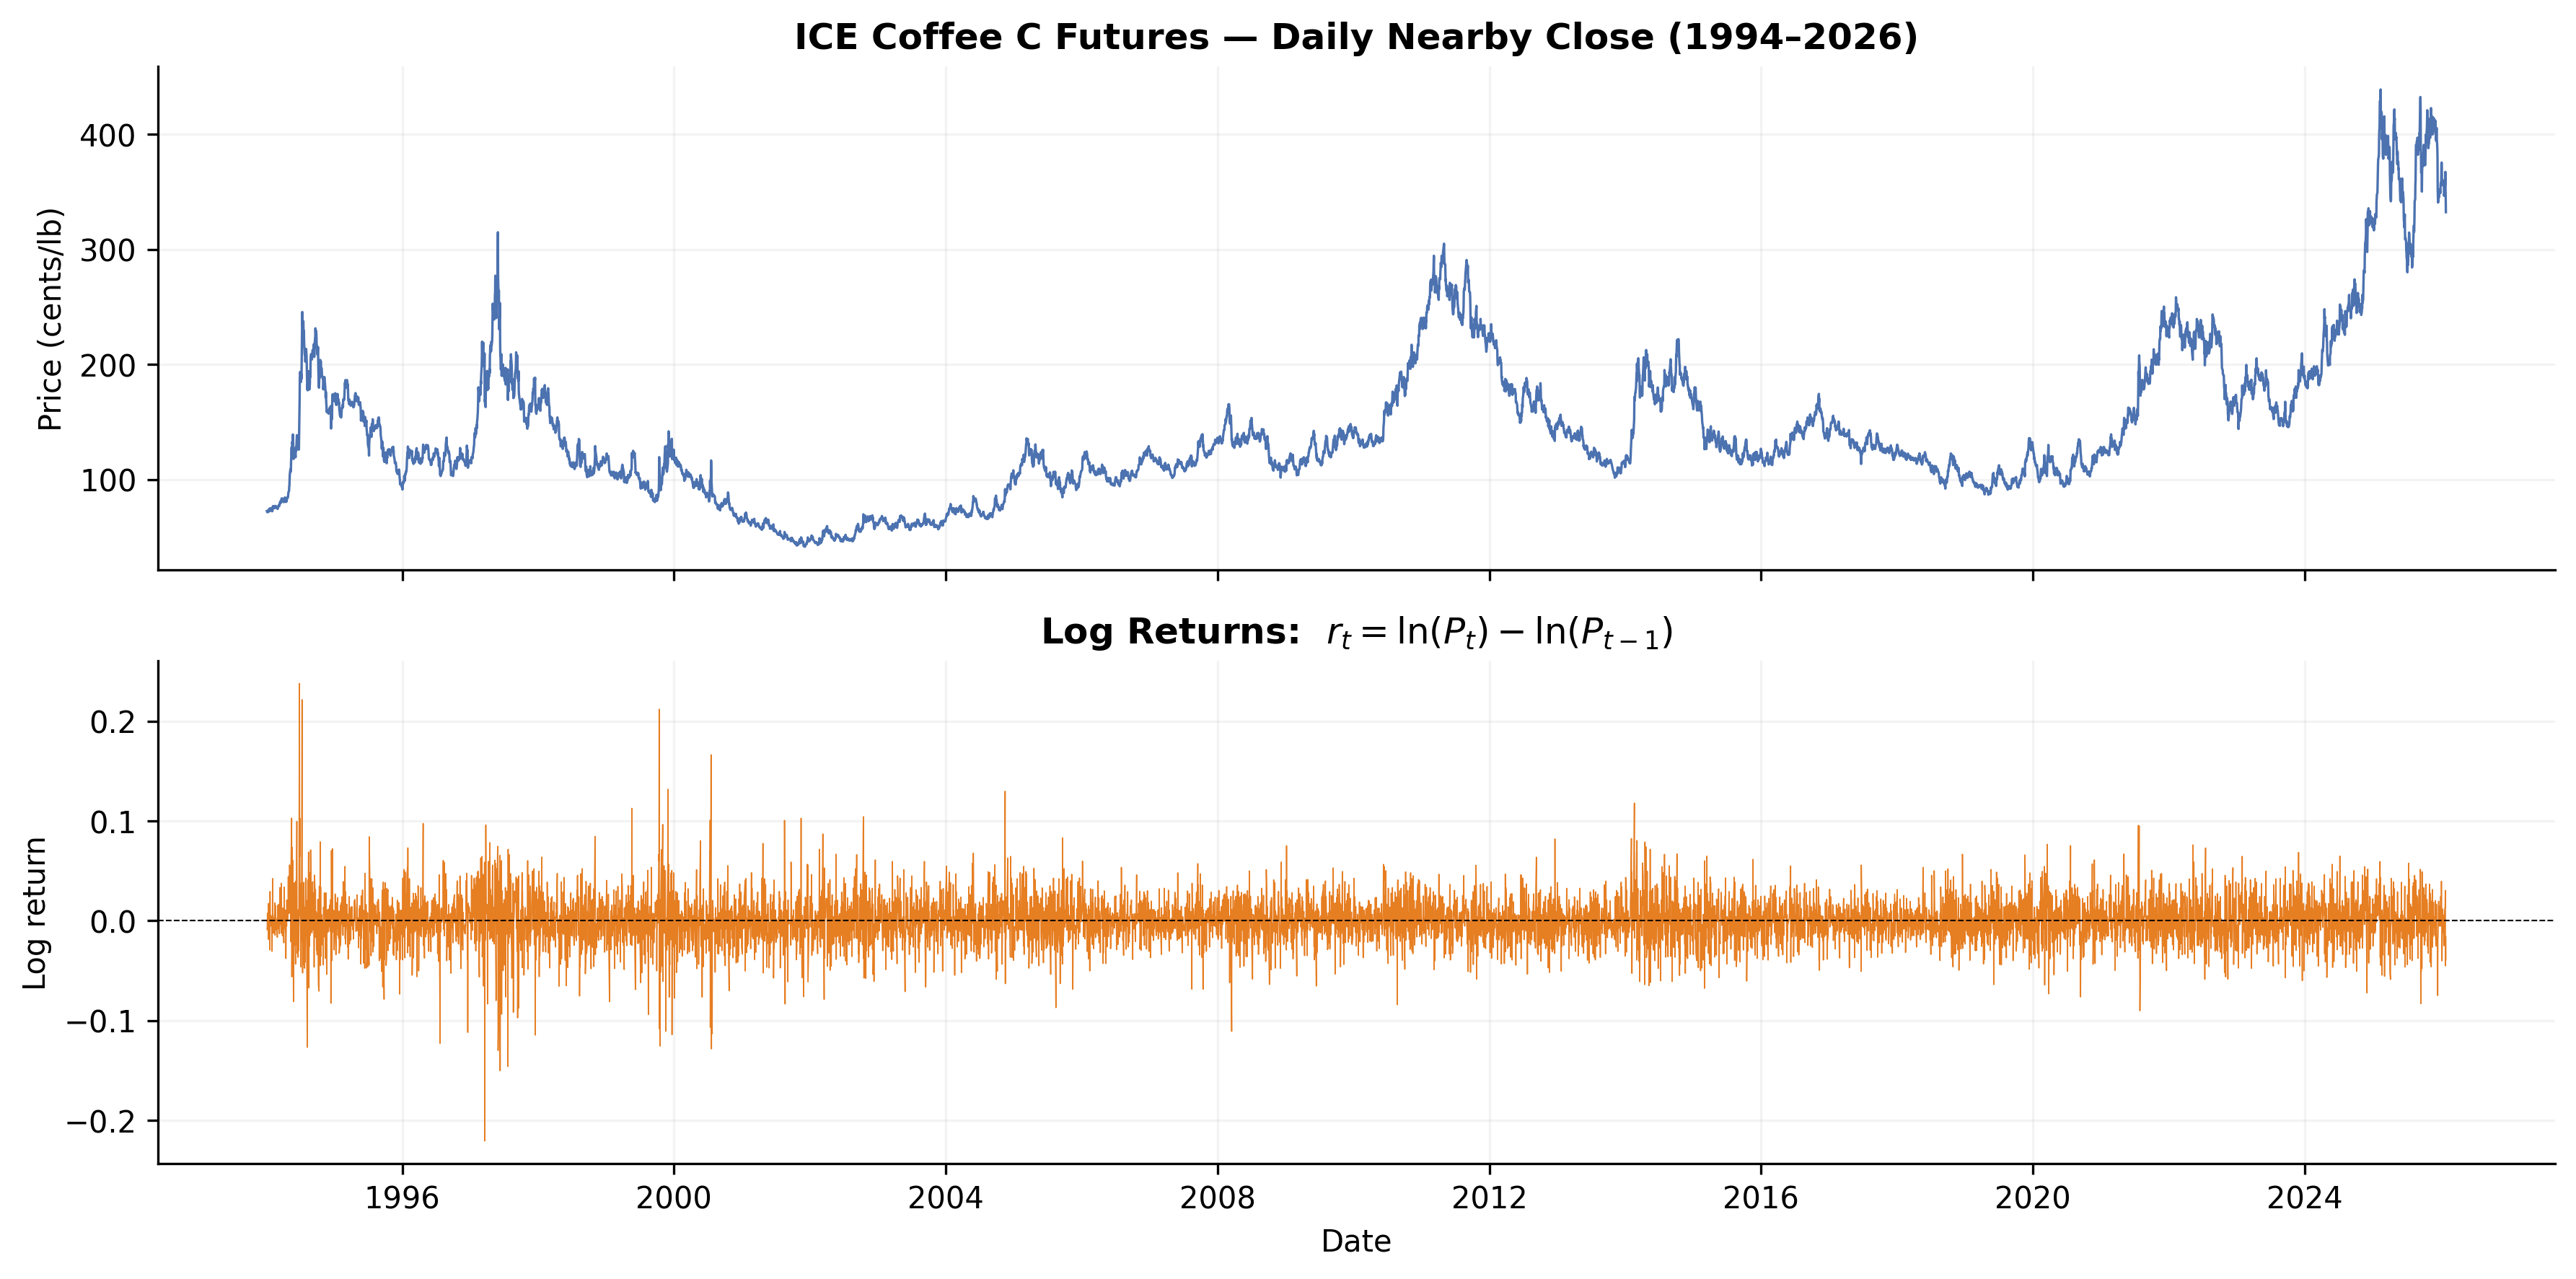
\includegraphics[width=\linewidth]{prices_vs_logreturns.png}
  \caption{(Top) ICE \emph{Coffee~C} nearby-close prices,
  1994--2026. (Bottom) Daily log-returns
  $r_t = \ln P_t - \ln P_{t-1}$. The mean of $r_t$ is
  $+1.9 \times 10^{-4}$ per day; visible heteroskedasticity around
  zero is the volatility-clustering pattern that motivates a
  GARCH-family model.}
  \label{fig:prices-vs-returns}
\end{figure}

\subsection{Linear predictability of returns}
\label{sec:linear-pred}

Under the weak form of market efficiency, daily returns should not be
linearly predictable from their own past. Two complementary tests
address this. Ljung-Box at $L \in \{10, 20\}$ formally rejects the
joint no-autocorrelation null ($p \approx 0.006$ at both lags), but
the underlying autocorrelations are economically negligible: the
mean of $|\hat\rho(k)|$ over lags 1--20 is approximately $0.013$,
with a maximum of $0.040$. This is the textbook stylized fact for
liquid financial returns \cite{cont2001empirical}: linear return
autocorrelations are statistically non-zero at very large $T$ but
too small to exploit through point-forecast models. The
heteroskedasticity-robust Lo-MacKinlay variance ratio
\cite{lo1988stock} provides a direct test of the random-walk
hypothesis robust to volatility clustering: across
$q \in \{2, 4, 8, 16, 32\}$, $\mathrm{VR}(q)$ stays within rounding
distance of 1 (from $0.986$ at $q=2$ to $0.852$ at $q=32$) and no
$z$-statistic reaches conventional significance. The variance ratio
fails to reject the random-walk null at every tested horizon---the
strongest direct evidence in the battery that the series is
consistent with a random walk.

\subsection{Long memory}
\label{sec:lr-hurst}

The Hurst exponent $H$ is estimated from the log-log slope of the
rescaled range, $\mathbb{E}[(R/S)_n] \sim c \cdot n^H$
\cite{hurst1951long}; $H = 0.5$ corresponds to no exploitable memory.
Classical $H$ is biased upward by short-range autocorrelation, so we
also compute Lo's modified R/S statistic $V_n$ \cite{lo1991long},
which applies a Bartlett-kernel HAC adjustment and has 95\%
acceptance region $V_n \in [0.809, 1.862]$ under the long-memory
null. We use the rule-of-thumb truncation lag
$q = \lfloor T^{1/3} \rfloor$ ($q = 20$ at $T = 8{,}103$) as an
alternative to the Andrews bandwidth
\cite{andrews1991heteroskedasticity}, with $V_n$ inside the
acceptance region under both choices. We find $H = 0.535$ and
$V_n = 1.137$: the Hurst estimate sits just above the random-walk
value, but the modified $V_n$ does not reject the no-long-memory
null. The $0.035$ excess of $H$ above $0.5$ is plausibly explained
by the small short-range autocorrelations of
Section~\ref{sec:linear-pred}, which classical $H$ is known to
absorb.

\subsection{Exploratory cross-checks}
\label{sec:exploratory}

To check the standard-battery conclusion from independent angles, we
also computed three metrics from the nonlinear-dynamics and
signal-processing literatures. All three converge with the standard
battery. Spectral mass on log-returns sits at the white-noise floor
($\Omega \approx 0.05$, against $0.68$ on price levels, where the
apparent ``structure'' is the I(1) drift signature rather than
exploitable periodicity). Permutation entropy sits near the
maximum-randomness ceiling on both representations ($0.97$ on prices,
$\approx 1.00$ on log-returns). The raw Lyapunov estimate
($\lambda = +0.071$) is indistinguishable from the shuffled-return
surrogate distribution (one-sided $p = 0.97$), consistent with
finite-sample bias of the Rosenstein algorithm on stochastic data
rather than with deterministic chaos. Implementation details, the
multi-frequency robustness check, and a discrete-length adaptation
of $\Omega$ that replaces the original $\log(2\pi)$ denominator with
$\log N_\mathrm{freq}$ to keep the metric in $[0, 1]$ at long series
are available in the project repository \cite{brinkman2026repo}.

\subsection{Synthesis}

Every diagnostic in Table~\ref{tab:diagnostics} points the same way:
the series carries no exploitable structure at this horizon that
simple baselines and complex models alike could extract, which is the
empirical signature of weak-form market efficiency
\cite{fama1970efficient} and is consistent with a random walk. The
prediction is therefore that any model in this class should be
roughly competitive with a random-walk baseline; the benchmark in
Sections~\ref{sec:backtest}--\ref{sec:stat-tests} confirmed that
prediction.

% ===================================================================
\section{Volatility Model for Prediction Intervals}
\label{sec:garch}
% ===================================================================

If point forecasts from the suite are statistically indistinguishable,
the deployment model must be chosen on a different basis. Coffee
returns exhibit pronounced volatility clustering (Fig.~\ref{fig:acf})
and heavy tails; both features make calibrated prediction intervals
non-trivial. The constant-variance bands a simple model would produce
are wrong in two directions at once---too wide in calm regimes,
too narrow in stressed ones. We adopt a GJR-GARCH(1{,}1) model with
constant mean and Student-$t$ innovations as the deployment
specification, following the standard framework for daily-frequency
financial-return modeling \cite{tsay2010analysis}. Each modeling
choice below is justified by a test on the same dataset; the section
walks through each in turn.

\subsection{Specification choices: mean, distribution, ARCH effects}

\emph{Mean.} A HAC-robust regression of log-returns on a constant
returns a daily mean of $+1.88 \times 10^{-4}$ with Newey-West
standard error $2.55 \times 10^{-4}$ (10 lags), $t = +0.74$,
$p = 0.46$. The drift is not statistically distinguishable from
zero, so we adopt a constant-mean specification.

\emph{Innovation distribution.} Daily log-returns have sample
skewness $+0.19$ and excess kurtosis $+6.65$. Jarque-Bera
\cite{jarque1980efficient} rejects normality at the limit of
numerical precision ($JB = 1.5 \times 10^4$, $p < 10^{-300}$). A
maximum-likelihood fit of the Student-$t$ distribution to the raw
returns yields $\nu \approx 4.2$, indicating substantially heavier
tails than Normal. We use Student-$t$ innovations.

\emph{ARCH effects.} Engle's ARCH LM test
\cite{engle1982autoregressive} with 10 lags yields $LM = 523.2$,
$p \approx 5 \times 10^{-106}$: the null of no conditional
heteroskedasticity is rejected at any reasonable significance level.
Fig.~\ref{fig:acf} contrasts the ACF of returns with the ACF of
squared returns: returns are nearly white noise, while squared
returns are persistently autocorrelated out to dozens of
lags---volatility clustering, the empirical pattern GARCH is
designed to capture.

\begin{figure}[t]
  \centering
  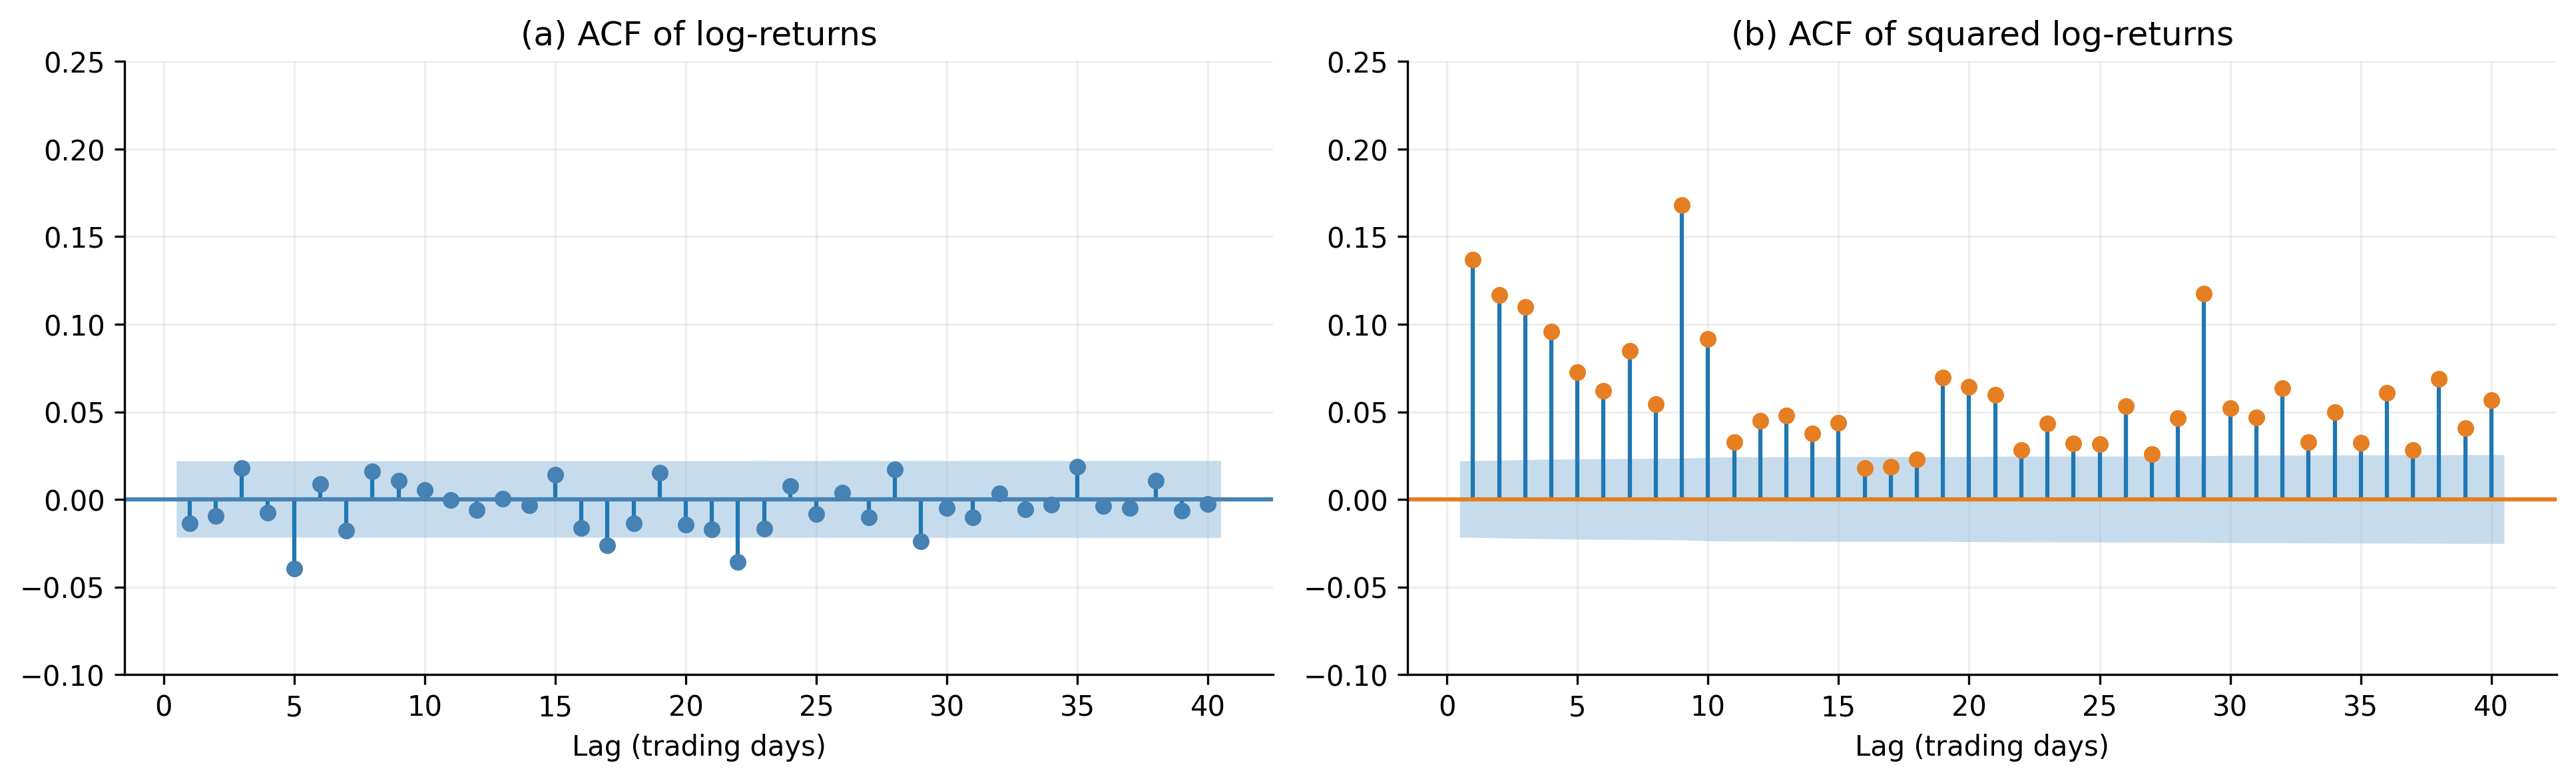
\includegraphics[width=\linewidth]{acf_returns_vs_squared.png}
  \caption{ACF of log-returns (left) and squared log-returns (right)
  for coffee. Returns are nearly white noise; squared returns are
  persistently autocorrelated, the textbook fingerprint of
  conditional heteroskedasticity.}
  \label{fig:acf}
\end{figure}

\subsection{Symmetric versus asymmetric volatility}

GARCH(1{,}1) \cite{bollerslev1986generalized} sets
$h_t = \omega + \alpha\, \varepsilon_{t-1}^2 + \beta\, h_{t-1}$.
GJR-GARCH \cite{glosten1993relation} adds an asymmetry term:
\[
  h_t = \omega + \alpha\, \varepsilon_{t-1}^2
       + \gamma\, \mathbb{1}_{\{\varepsilon_{t-1} < 0\}}\, \varepsilon_{t-1}^2
       + \beta\, h_{t-1},
\]
allowing negative and positive shocks of equal magnitude to
contribute differently to next-period variance.

Fitting both specifications to the full sample yields:

\begin{itemize}
  \item \textbf{GARCH(1{,}1)-t}: $\mathrm{AIC} = 35492.7$,
    $\mathrm{BIC} = 35527.7$; Ljung-Box on squared standardized
    residuals $p_{LB(10)} = 0.0003$, $p_{LB(20)} = 0.0010$.
  \item \textbf{GJR-GARCH(1{,}1)-t}: $\mathrm{AIC} = 35450.4$,
    $\mathrm{BIC} = 35492.4$; Ljung-Box on squared standardized
    residuals $p_{LB(10)} = 0.048$, $p_{LB(20)} = 0.093$.
\end{itemize}

GJR improves AIC by 42 and BIC by 35; the Ljung-Box squared-residual
p-values climb by roughly two orders of magnitude at both lag
choices. $LB(10)$ remains just under 0.05, indicating some residual
structure at short lags; $LB(20)$ clears 0.05. We adopt
GJR-GARCH(1{,}1)-t as a defensible complexity/fit trade-off.

\subsection{Fitted-parameter diagnostics}

The fitted leverage parameter is $\gamma = -0.058$, statistically
distinguishable from zero ($p < 0.001$). For equities, the GJR
leverage parameter is typically positive: negative price shocks
increase volatility more than positive shocks of equal size (the
"leverage effect"). The sign on coffee is reversed: positive return
shocks inflate volatility more than negative ones. This is plausible
for soft commodities where supply-disruption events (frost, drought,
geopolitical) coincide with the largest upward price jumps;
"good news for the price" and "bad news for the supply" arrive
together, and both inflate volatility.

Volatility persistence is
$\alpha + \gamma/2 + \beta = 0.973$, corresponding to a half-life of
volatility shocks of approximately 26 days---typical for daily
commodity volatility, with persistence below 1 (the stability
condition for unconditional variance to exist). The fitted Student-$t$
degrees of freedom on standardized residuals is $\nu \approx 5.7$,
higher than the $\nu \approx 4.2$ obtained from the raw-return fit
in the distribution section. The two values are not in conflict:
they measure different quantities. The raw-return $\nu$ captures the
tail thickness of \emph{unconditional} returns, which inherits heavy
tails partly from volatility clustering itself; the residual $\nu$
captures the tail thickness of innovations \emph{after} GJR-GARCH
absorbs the time-varying variance. Once that variance is filtered
out, the residual distribution looks closer to Normal, although
still heavy enough that Student-$t$ innovations are required.

\subsection{Conditional versus constant-variance intervals}

Fig.~\ref{fig:bounds} contrasts the constant-variance
$\pm 1.96 \hat\sigma$ band against the GJR-GARCH conditional
$\pm 1.96 \sigma_t$ band, overlaid on the realized log-returns. Both
bands achieve roughly 95\% unconditional coverage in-sample, but the
\emph{when} differs. The constant band is too wide in calm regimes
(2002--2005, 2017--2019), wasting precision when realized volatility
is low, and too narrow in stressed regimes (1997 frost, 2010--2011
rally, 2024--2025 rally), failing to cover when realized volatility
spikes. The conditional band expands and contracts with realized
volatility, which is the difference between useful and misleading
intervals for downstream procurement decisions.

\begin{figure}[t]
  \centering
  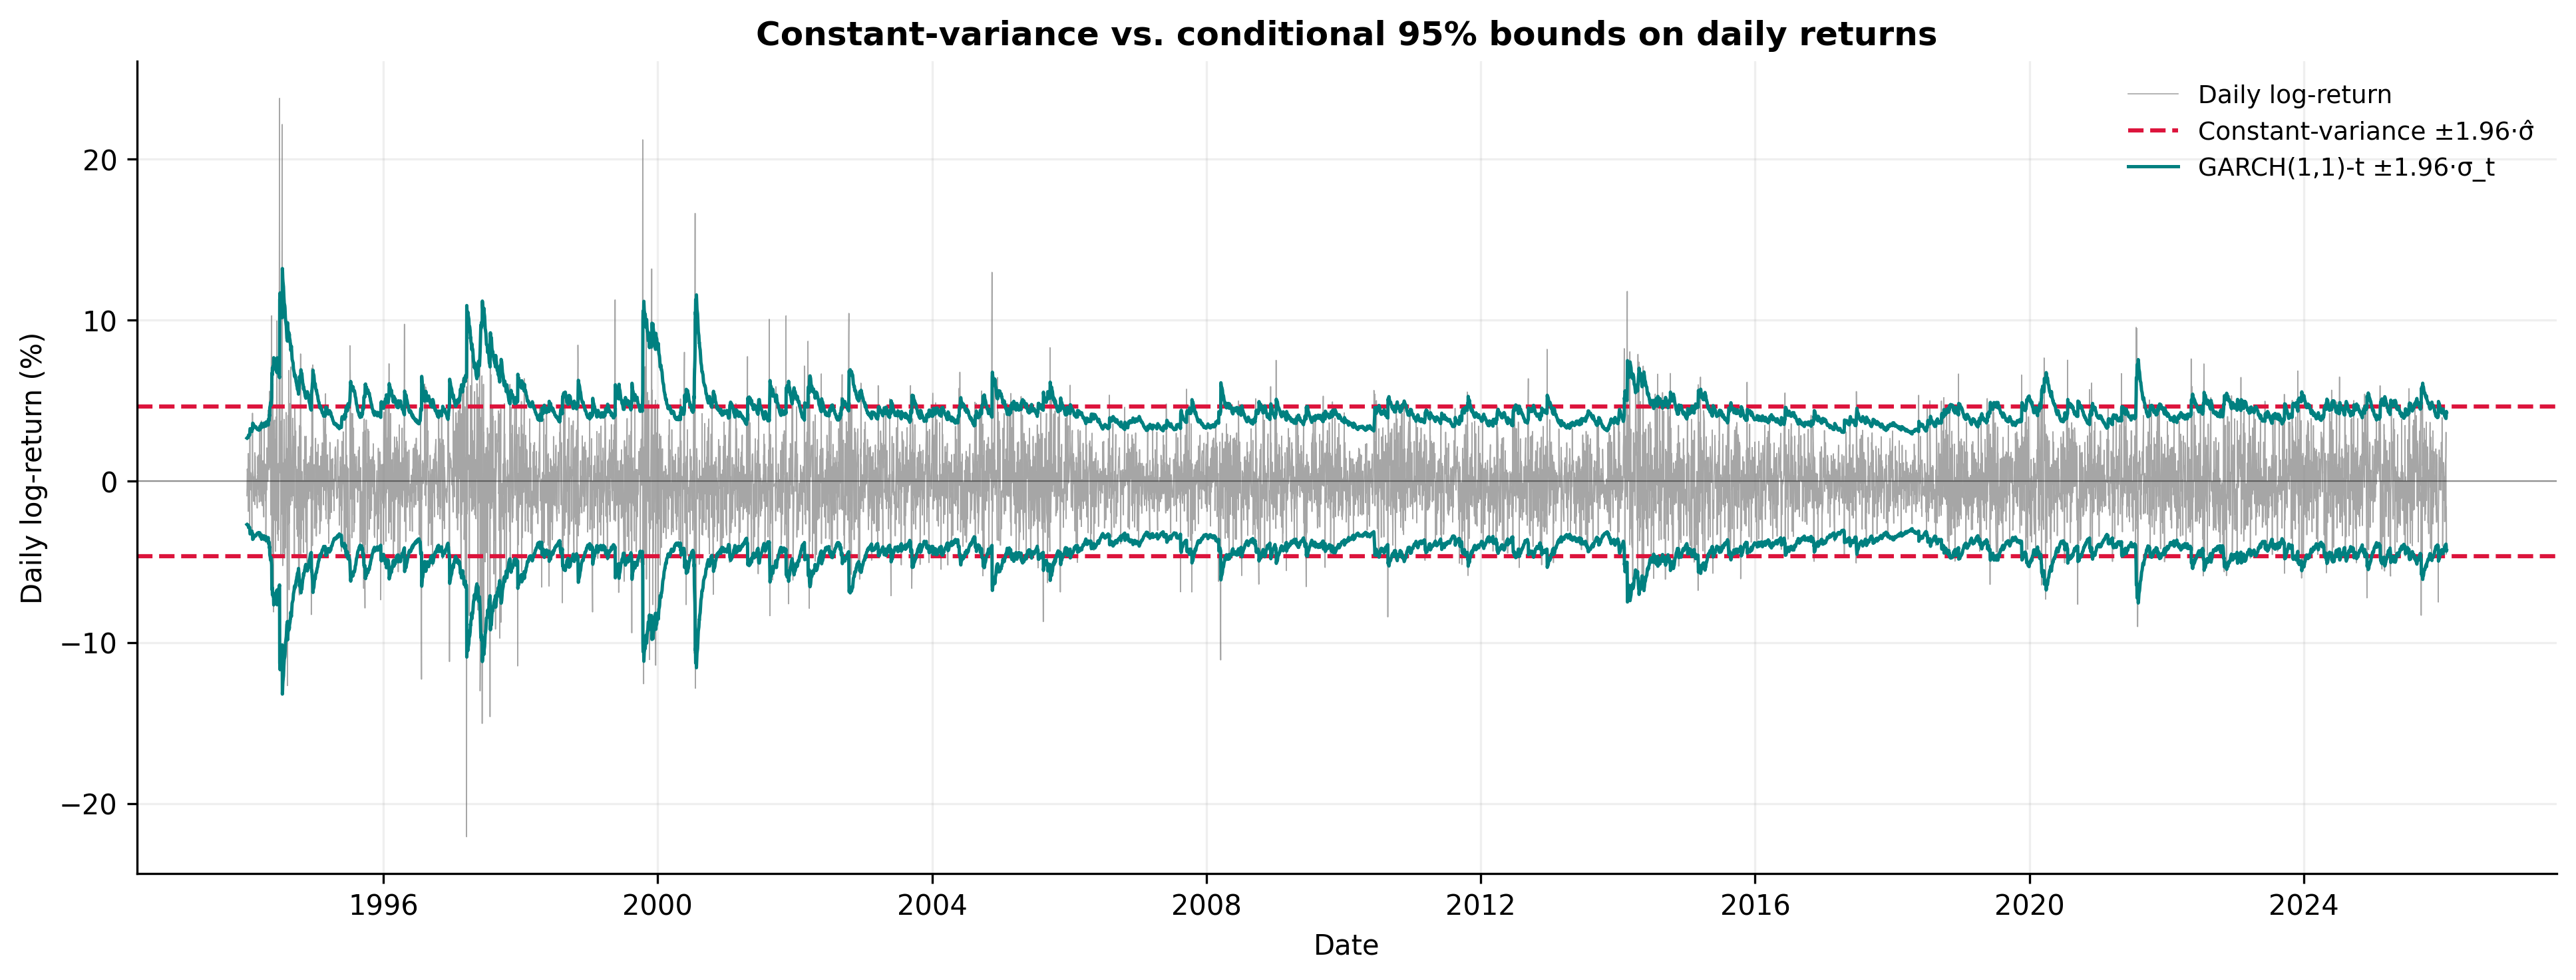
\includegraphics[width=\linewidth]{constant_vs_conditional_bounds.png}
  \caption{Constant-variance $\pm 1.96 \hat\sigma$ band (red,
  horizontal) versus GJR-GARCH conditional $\pm 1.96 \sigma_t$ band
  (teal) on daily log-returns. Both achieve $\approx 95\%$
  unconditional coverage; the conditional band adapts to regime,
  expanding during stress periods and narrowing during calm.}
  \label{fig:bounds}
\end{figure}

\subsection{Out-of-sample coverage}

Specification tests show the model fits in-sample; the operational
question is whether its prediction intervals are calibrated
out-of-sample. We refit GJR-GARCH(1{,}1)-t at the same 60 evenly-spaced
origins used in the Section~\ref{sec:backtest} benchmark, this time
on \emph{expanding} windows (all history up to each origin). Expanding
rather than rolling windows stabilizes the Student-$t$ degrees-of-freedom
estimate, which is notoriously sample-sensitive; across the 60 origins
$\nu$ has median $4.79$, range $[4.18, 5.64]$, and standard deviation
$0.43$. At each origin we produce 63-step forecasts of the conditional
variance, integrate to cumulative variance, and back out 80\% and 95\%
prediction intervals on prices using the Student-$t$ quantiles. We
then count the fraction of realized prices that fall inside each band
at each step.

\begin{figure}[t]
  \centering
  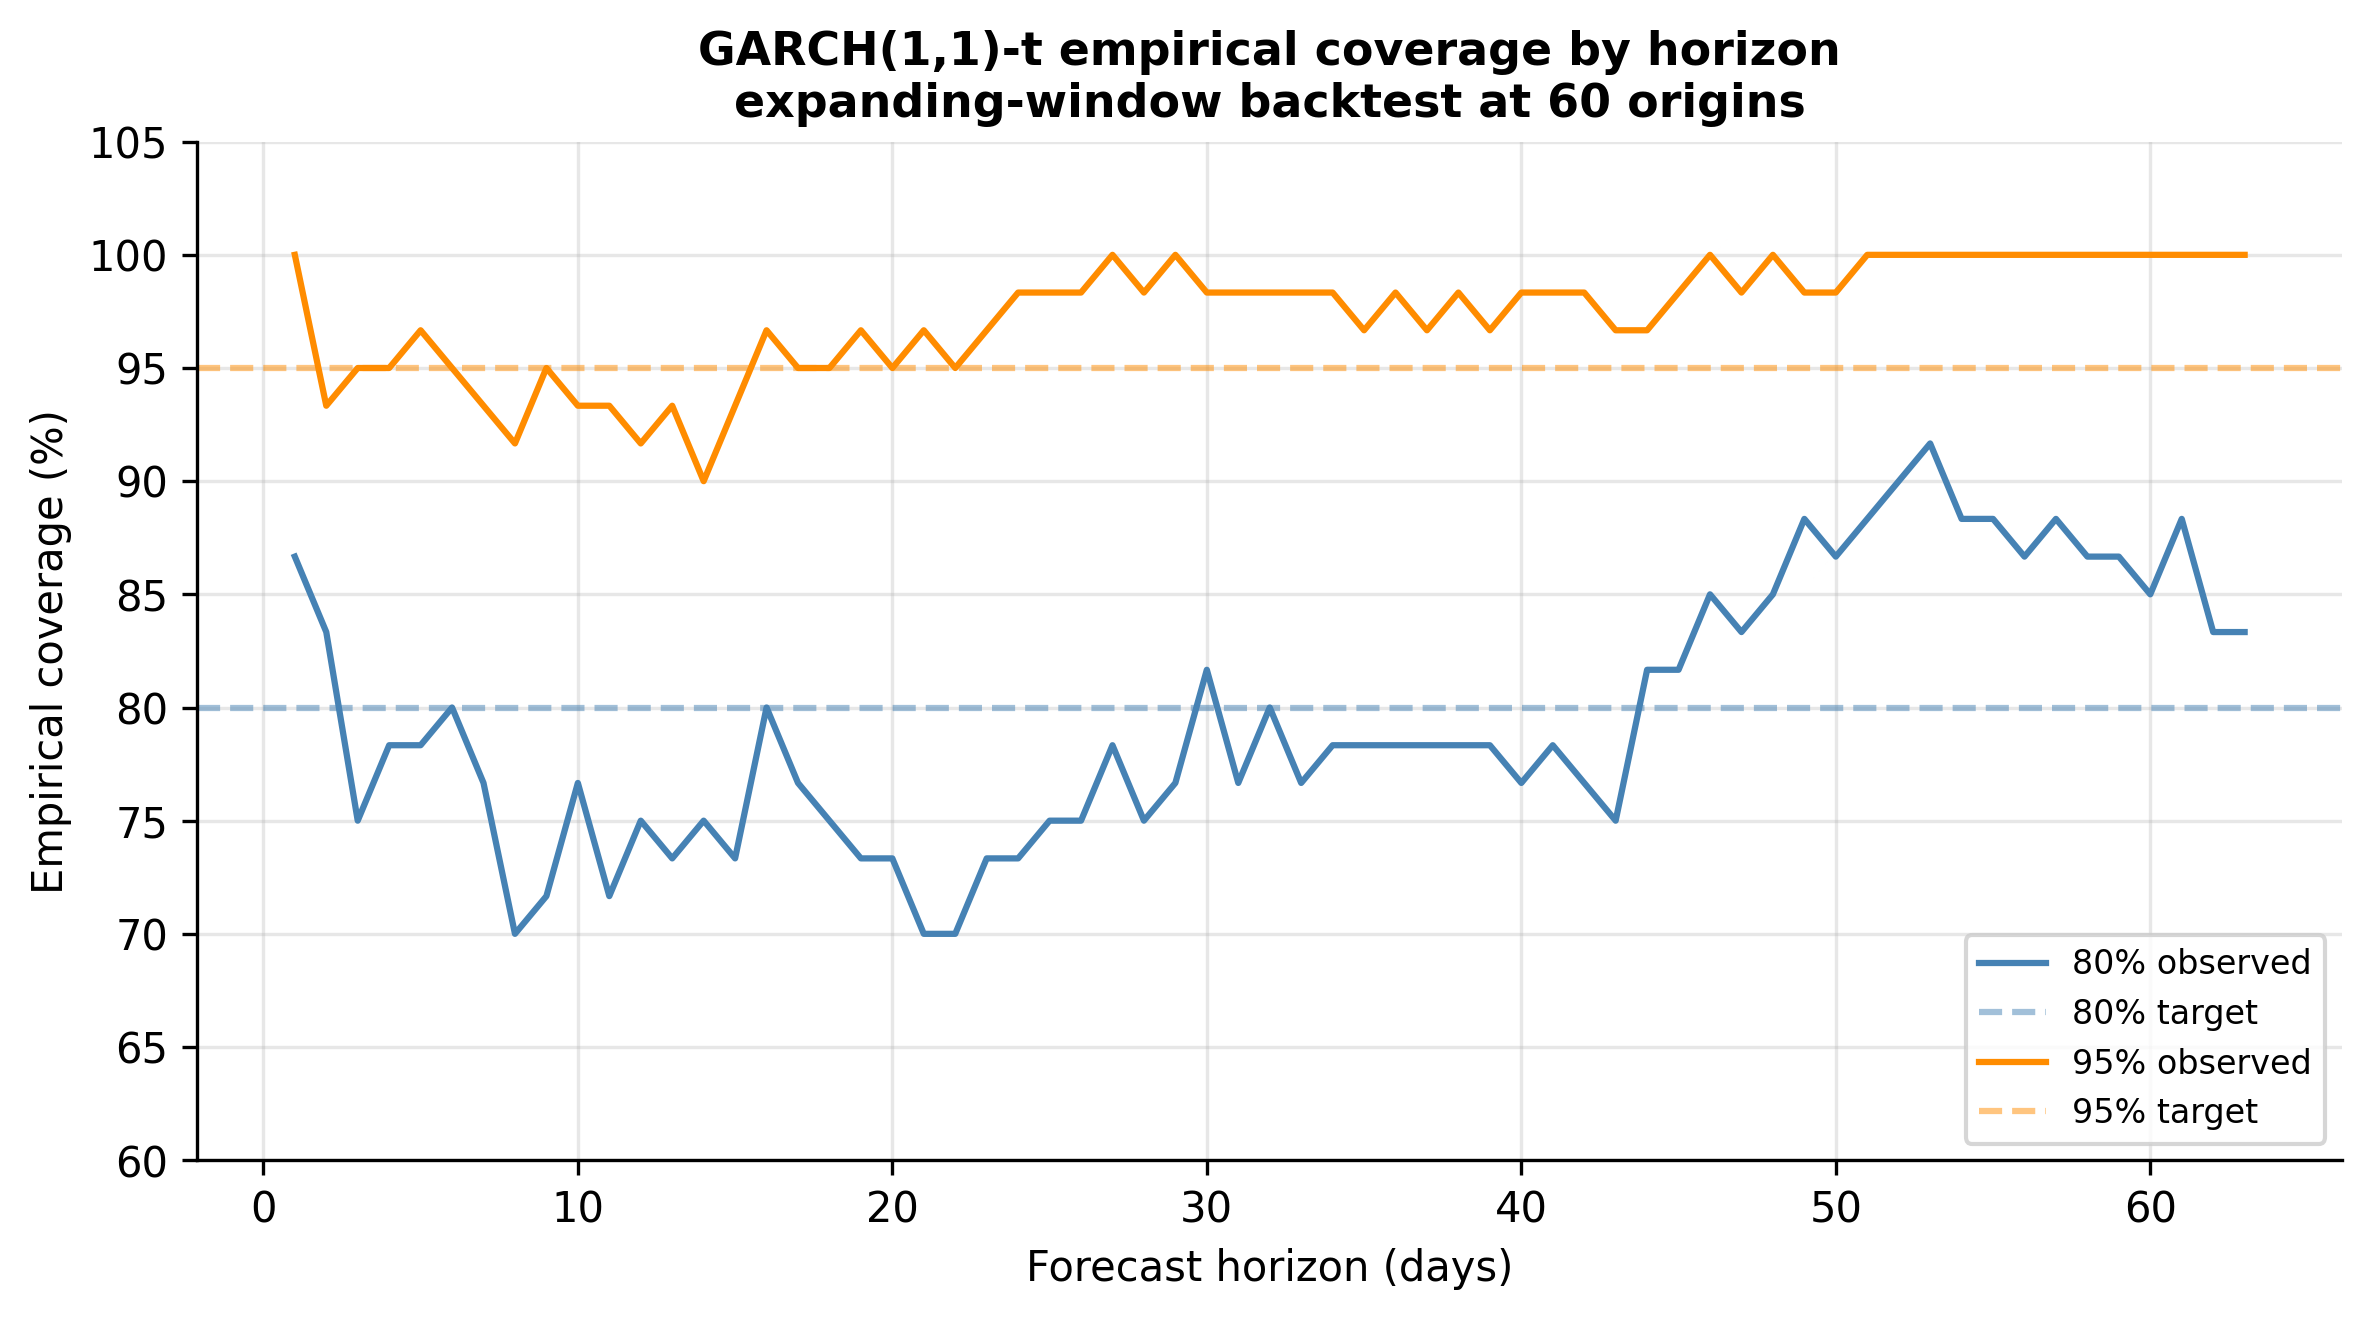
\includegraphics[width=\linewidth]{garch_coverage.png}
  \caption{Empirical coverage of GJR-GARCH(1{,}1)-t prediction
  intervals across 60 expanding-window origins, by horizon step.
  Solid lines: observed coverage; dashed: nominal 80\% and 95\%
  targets. The 95\% interval is at or above nominal across the full
  horizon; the 80\% interval undercovers by 2--10 percentage points
  through the first month and recovers to meet or exceed nominal
  thereafter.}
  \label{fig:garch-cov}
\end{figure}

Fig.~\ref{fig:garch-cov} shows the result. The 95\% interval meets
or slightly exceeds nominal across the full 63-day horizon---safely
conservative, the direction a deployment forecast wants to err. The
80\% interval is less uniform: it sits around 73--78\% through the
first month, with a minimum near 70\% at horizon 14, before rising
to meet or exceed 80\% from roughly horizon 45 onward. The pattern
is consistent with the model's short-horizon variance being slightly
under-dispersed; the practical consequence for a procurement reader
is that the 80\% band over the first month is closer to a
\textit{75\% band}, while the 95\% band is reliable throughout.

Fig.~\ref{fig:garch-samples} provides a qualitative complement: six
origins drawn from the 60, each showing the realized path against the
point forecast and the 80\% and 95\% intervals. The realized path
stays inside the 95\% band at all six origins and inside the 80\%
band most of the time, including across the high-volatility 2011
episode (Origin~26) and the 2024--2025 rally (Origin~59).

\begin{figure*}[t]
  \centering
  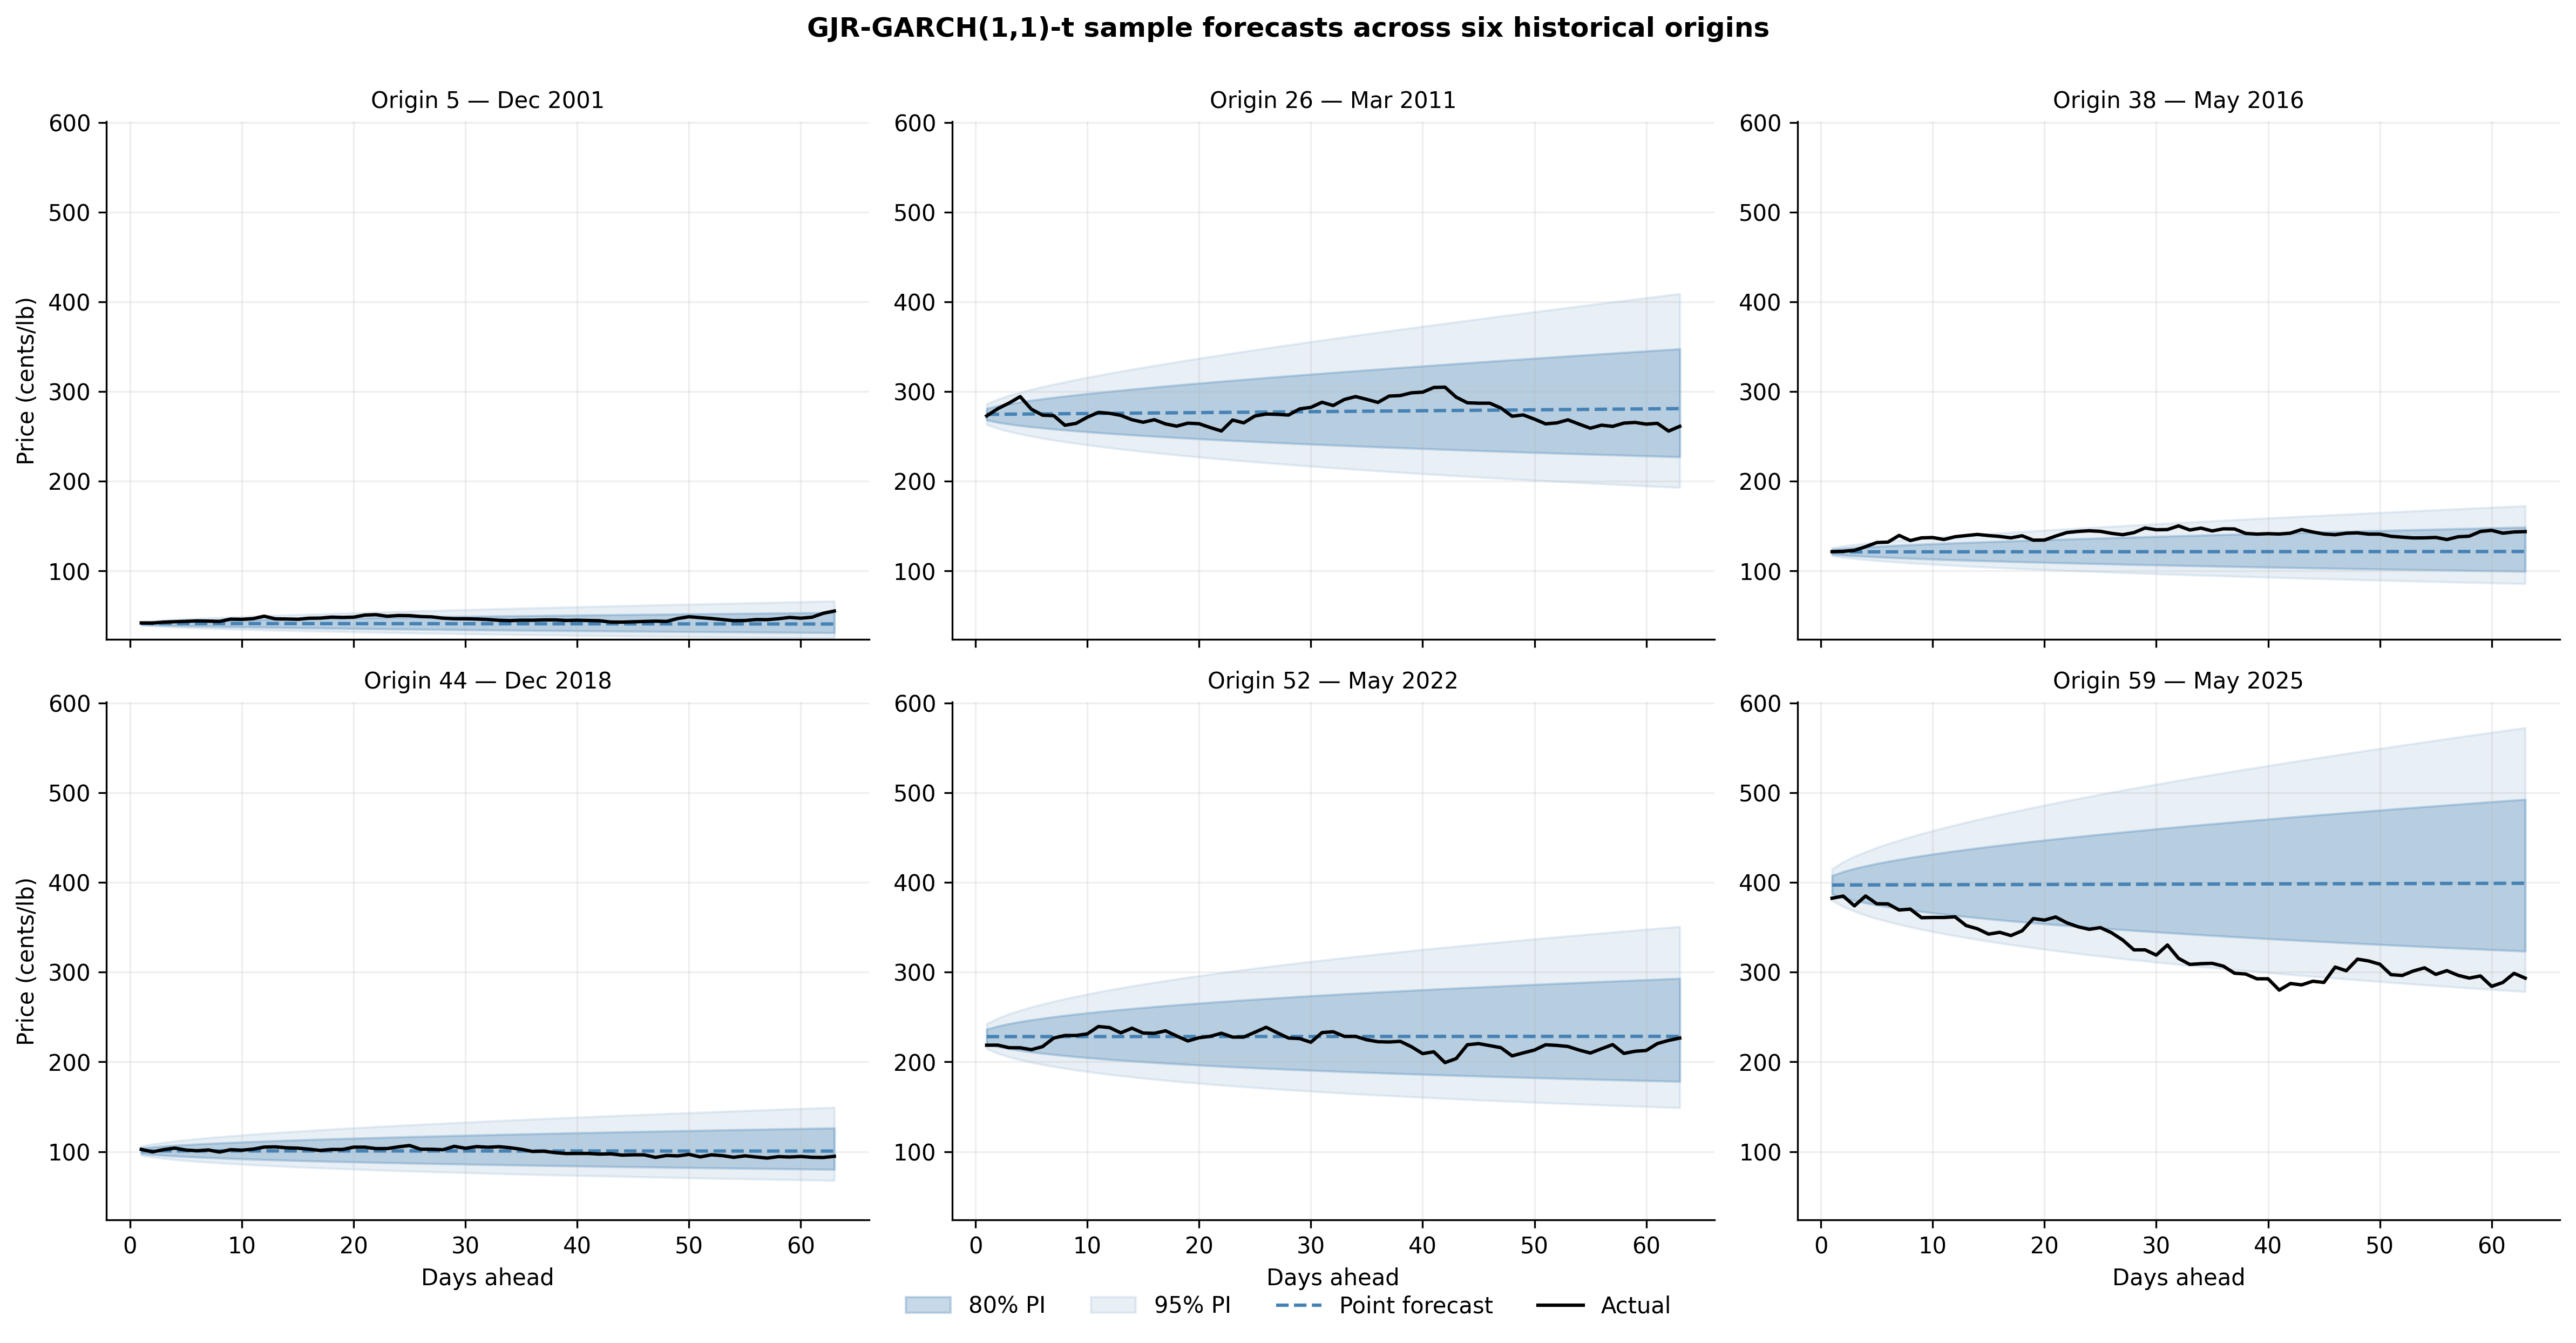
\includegraphics[width=\linewidth]{garch_sample_forecasts.png}
  \caption{Six sample GJR-GARCH(1{,}1)-t forecasts drawn from the
  60-origin backtest. Each panel shows the realized 63-day path
  (black) against the point forecast (dashed) and the 80\% and 95\%
  prediction intervals (shaded), produced by an expanding-window
  refit at the indicated origin date.}
  \label{fig:garch-samples}
\end{figure*}

\subsection{Summary and scope of the specification search}

Table~\ref{tab:garch-decisions} collects the specification choices
and the test that justifies each.

\begin{table}[t]
\caption{GJR-GARCH(1{,}1)-t specification choices}
\label{tab:garch-decisions}
\centering
\renewcommand{\arraystretch}{1.15}
\begin{tabular}{@{}p{0.45\linewidth}p{0.45\linewidth}@{}}
\toprule
\textbf{Decision} & \textbf{Justified by} \\
\midrule
Model log-returns, not prices    & ADF, KPSS, PP (Sec.~\ref{sec:stationarity}) \\
Constant mean, not AR            & HAC $t$-stat $|t| = 0.74$, $p = 0.46$ \\
Student-$t$, not Normal          & Excess kurtosis $6.65$; Jarque-Bera \\
GARCH family over IID            & ARCH LM, $p \approx 5 \times 10^{-106}$ \\
GJR over plain GARCH             & AIC, BIC, squared-residual LB \\
Expanding-window fits            & Stabilizes $\nu$; calibrated coverage \\
80\% / 95\% PIs                  & 95\% at/above nominal; 80\% near 75\% early, recovers later \\
\bottomrule
\end{tabular}
\end{table}

GJR-GARCH(1{,}1)-t is presented here as an \emph{informed} choice
within the broader GARCH family rather than the optimum of an
exhaustive specification search. We compared the chosen model against
plain GARCH(1{,}1)-t and verified it on the standard diagnostic
ladder (drift, distribution, ARCH effects, asymmetry, residual
autocorrelation, out-of-sample coverage), but did not evaluate
alternative volatility families such as EGARCH, FIGARCH, component
GARCH, stochastic-volatility, or HAR-RV models. A more thorough
specification search may yield marginal improvements in coverage or
tightness; the chosen specification is the one that satisfies the
in-sample diagnostics and the out-of-sample 80\% / 95\% coverage
targets the procurement use-case requires, with the lowest complexity
that does so.

% ===================================================================
\section{Deployment}
\label{sec:deployment}
% ===================================================================

The GJR-GARCH(1{,}1)-t model is operationalized as a daily forecast
running on a scheduled GitHub Actions cron. Each invocation loads the
committed historical series, appends any newer ICE \emph{Coffee~C}
closes from Yahoo Finance (ticker \texttt{KC=F}), refits the model
on log-returns, and writes a 63-day forecast with 50\%, 80\%, and
95\% intervals to a CSV plus a PNG plot. The latest run is held at a
fixed path and each daily run is archived in a
year/month-organized directory for traceability. The pipeline is
reproducible from a fresh clone; full source, the model package, and
the four analysis notebooks are publicly available
\cite{brinkman2026repo}.

Fig.~\ref{fig:live} shows the production forecast at the time of
writing: the recent observed price path, the GJR-GARCH(1{,}1)-t point
forecast, and the 50\%, 80\%, and 95\% prediction intervals over the
63-day horizon. The image is regenerated by every scheduled run and
serves as the visible artifact of the deployed system.

\begin{figure}[t]
  \centering
  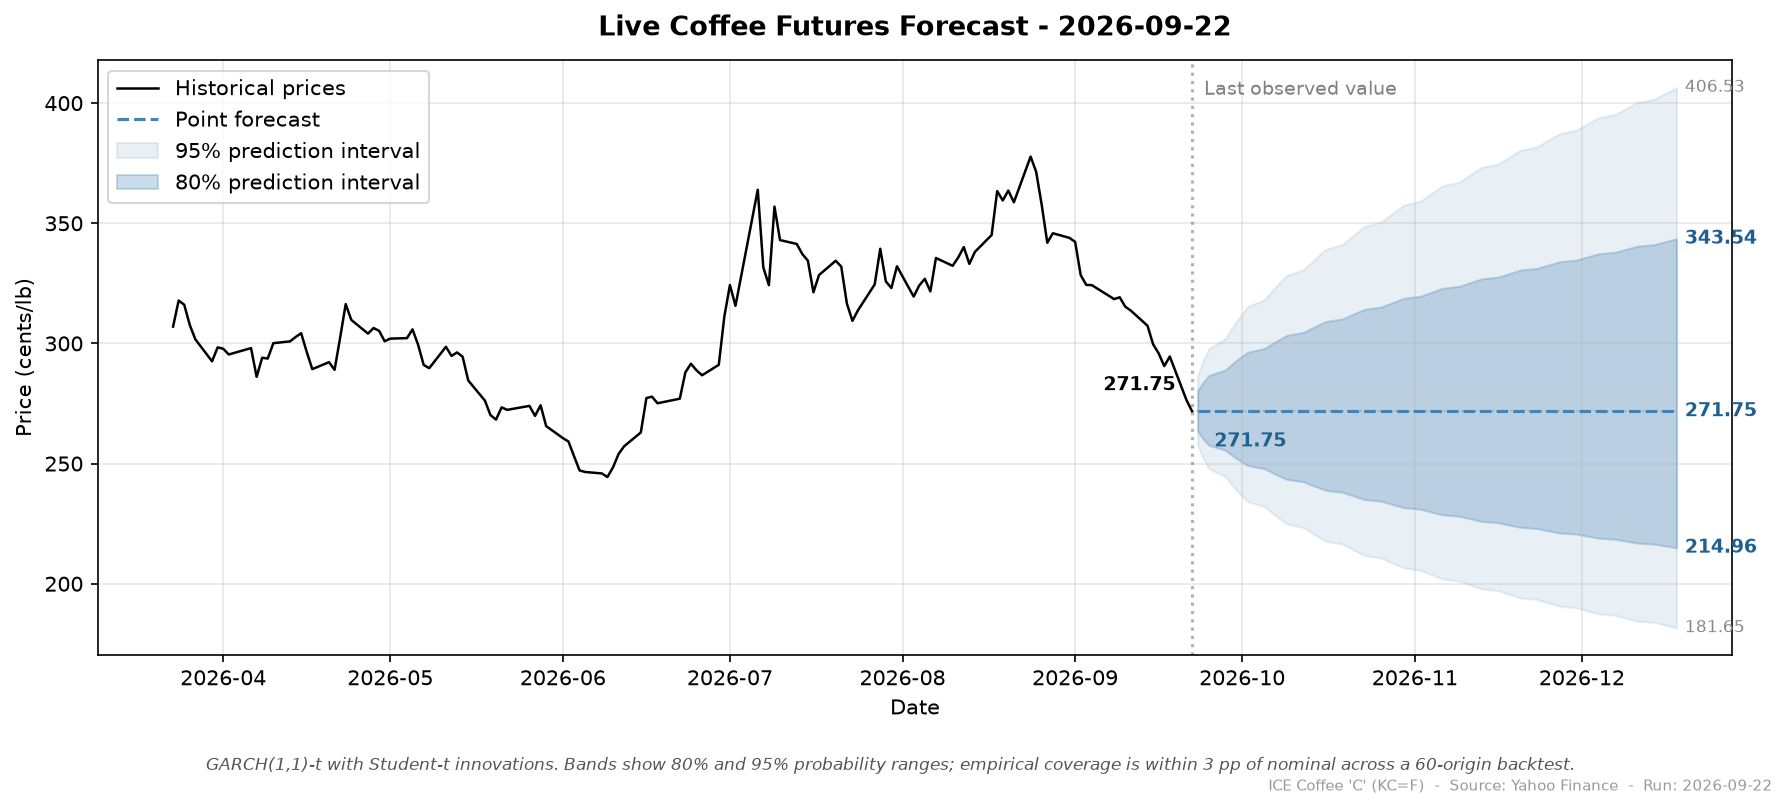
\includegraphics[width=\linewidth]{latest_forecast.png}
  \caption{Production output of the deployed pipeline at the time of
  writing: ICE \emph{Coffee~C} nearby-close history (left of the
  vertical separator), the GJR-GARCH(1{,}1)-t point forecast, and
  the 50\%, 80\%, and 95\% prediction intervals over the next 63
  trading days. The image is overwritten on every scheduled run
  of the daily pipeline.}
  \label{fig:live}
\end{figure}

% ===================================================================
\section{Conclusion}
\label{sec:conclusion}
% ===================================================================

We benchmarked ten forecasting models spanning five methodological
categories on 32 years of ICE \emph{Coffee~C} nearby-close daily
prices. The 60-origin rolling-window backtest, the Diebold-Mariano
test against a random-walk baseline, and the Hansen-Lunde-Nason
Model Confidence Set all converge on the same finding: nine of the
ten models are jointly indistinguishable in terms of point-forecast
accuracy at $\alpha = 0.10$, including a pretrained foundation model
fed a six-year context window. Only Prophet falls outside the
confidence set.

The model-free forecastability battery explains why. ADF, KPSS, and
Phillips-Perron place the series on a unit root; the
heteroskedasticity-robust Lo-MacKinlay variance ratio fails to
reject the random-walk null at every tested horizon; the Hurst
exponent is just above $0.5$ but Lo's modified $V_n$ does not
reject no-long-memory; spectral predictability on log-returns is
near the white-noise floor; permutation entropy is near the ceiling
on both representations; and the raw Lyapunov exponent is
statistically indistinguishable from that of shuffled returns. The
collective signature is one of no exploitable structure at this
horizon---consistent with weak-form market efficiency, and with a
random walk as the simplest model that fits.

Because the benchmark's point-forecast accuracies are
indistinguishable, the deployment model is chosen on the basis of
prediction intervals. A GJR-GARCH(1{,}1)-t model with constant mean
and Student-$t$ innovations is justified specification-by-specification
through HAC-robust drift tests, the ARCH LM test, AIC/BIC comparisons
against plain GARCH, and Ljung-Box on squared standardized residuals.
An expanding-window backtest at 60 historical origins confirms 95\%
empirical coverage at or above nominal across the full 63-day
horizon, with 80\% coverage approaching nominal by mid-horizon after
modest undercoverage in the first month. The deployed system produces a daily
forward distribution that is appropriate for the procurement use-case
that motivated the project.

\section*{Acknowledgments}

This work was completed as a semester project for MATH 1103,
\emph{Mathematical Problems in Business, Industry, and Government}
(also known as ``Big Problems''), Department of Mathematics,
University of Pittsburgh, in collaboration with 19 Coffee Company.
The authors thank Dr.~Jeffrey Paul Wheeler for instruction and
guidance throughout the project, and 19 Coffee Company for serving
as the project's stakeholder and providing the operational context
that shaped the deployment design.

\bibliographystyle{IEEEtran}
\bibliography{refs}

\end{document}